\documentclass[12pt,a4paper]{article}
\usepackage[page,header]{appendix}
\usepackage{lmodern}

%%%%%% TIKZ BIBLIOTHÈQUES %%%%%%
\usepackage{tikz}
\usetikzlibrary{3d}
\usepackage{pgfplots}
\usetikzlibrary{patterns}
\usepackage[european resistor, european voltage, european current]{circuitikz}
\usetikzlibrary{arrows,shapes,positioning}
\usetikzlibrary{decorations.markings,decorations.pathmorphing,
	decorations.pathreplacing}
\usetikzlibrary{calc,patterns,shapes.geometric}
\usepackage{tikz-3dplot}
\usetikzlibrary{matrix, calc, backgrounds, decorations.pathreplacing}
\usepackage{mathtools}
\usetikzlibrary{arrows.meta}

%%%%%%%%%%%%%%%%%%%%%%%%%%%%%%%

%%%%% GESTION DES RÉFÉRENCES %%%%%%
\usepackage{caption}
\pgfplotsset{compat=newest}
\usepackage{hyperref} % Crée des hyperliens pour le sommaire
\hypersetup{pdfborder=0 0 0} % Cache les cadres rouges autour des hyperliens
%%%%%%%%%%%%%%%%%%%%%%%%%%%%%%%%%%

%%% PAGE DE COUVERTURE %%%
\usepackage[utf8]{inputenc}
\usepackage[T1]{fontenc}
\usepackage[english]{babel}
%Includes "References" in the table of contents
\usepackage[nottoc]{tocbibind}
%%% GESTION DES FIGURES %%%
\usepackage{float}      % Pour les figures à la place voulue UNIQUEMENT
\usepackage{graphicx}   % Pour inclure des figures
\usepackage{chngcntr}   % Bibli pour que la numérotation des figures dépende de la section
\usepackage{fancyhdr}
\usepackage{geometry}
\usepackage{titlesec}
\usepackage{tocloft} % package to adjust the appearance of the table of contents.
\usepackage{titletoc}

\usepackage{lipsum} % for sample text
\usepackage{glossaries}

\usepackage{amsfonts}   % Ensemble mathématique
\usepackage{amsmath}    % Environnement mathématique équation
\usepackage{tabularx}
\usepackage{colortbl}
\usepackage{array}
\usepackage{tcolorbox} % box coloré
\tcbuselibrary{skins} % Utilse pour faire Titres avancés: Personnaliser l'emplacement et l'apparence des titres des boîtes bien au-delà des capacités de base, comme dans l'exemple que je vous ai fourni, où le titre est placé en chevauchement sur le bord supérieur de la boîte.
\usepackage{mdframed}   % Box Théorèmes et définitions
\usepackage{xspace}     % Pour les redéfinitions de commandes
\usepackage{makecell}   % Pour des retours à la ligne dans une ligne de tableau
\usepackage{physics} % notation mathématique pour la physique 
\usepackage{subcaption}
\usepackage{amsthm}
\usepackage{algorithm}
\usepackage{algpseudocode}

%%% CONFIGURATION DE LA PAGE %%%
\usepackage{fancyhdr}
\usepackage{geometry}
\usepackage{titlesec}
\usepackage{systeme}
\usepackage{palatino} %%% style of the Latex
\usepackage{lastpage} 


\hypersetup{
    colorlinks=true,
    linkcolor=blue,     % Color for internal links (sections, equations, etc.)
    urlcolor=magenta,       % Color for URLs
    citecolor=red,    % Color for citations
    filecolor=green   % Color for file links
}
\hypersetup{pdfborder=0 0 0} % Cache les cadres rouges autour des hyperliens
%%%%%%%%%%%%%%%%%%%%%%%%%%%%%%%%%%


%%% Section
\newcommand{\hugetext}[1]{%
  \begin{flushleft}
    {\huge \textbf{#1}}
  \end{flushleft}
}




%%%
% Redefine the abstract environment
\makeatletter
\renewenvironment{abstract}{
    \if@twocolumn
      \section*{\abstractname}%
    \else
      \begin{center}%
        {\Huge\bfseries \leftline{\abstractname\vspace{-1em}}\vspace{0.3em}}%
      \end{center}%
	  \noindent

    \fi}
    {\if@twocolumn\else\endquotation\fi}
\makeatother
%%% Redefine the Contents


%%% color %%%

%%% color %%%

\definecolor{asparagus}{rgb}{0.53, 0.66, 0.42}
\definecolor{carminered}{rgb}{1.0, 0.0, 0.22}
\definecolor{darkpastelblue}{rgb}{0.47, 0.62, 0.8}
\definecolor{darkgray}{rgb}{0.66, 0.66, 0.66}
\definecolor{harvardcrimson}{rgb}{0.79, 0.0, 0.09}
\definecolor{aurometalsaurus}{rgb}{0.43, 0.5, 0.5}
\definecolor{ashgrey}{rgb}{0.7, 0.75, 0.71}
\definecolor{citrine}{rgb}{0.89, 0.82, 0.04}
\definecolor{airforceblue}{rgb}{0.36, 0.54, 0.66}
\definecolor{applegreen}{rgb}{0.55, 0.71, 0.0}
\definecolor{burgundy}{rgb}{0.5, 0.0, 0.13}



%%%%CONFIG MATHS EQUATIONS
\usepackage{ mathrsfs } % FOR the H of the Hamiltionan

\newcommand{\id}[2]{ \hat{\mathbb{I}}_{#1}^{(#2)}}
\newcommand{\strope}[1]{ e^{i \pi \phi _{#1}}}
\newcommand{\stropeall}[1]{ e^{i \pi \displaystyle{ \sum_{l < #1}} f_l^\dagger f_l}}
\newcommand{\fd}[1]{ f^\dagger_{#1}}
\newcommand{\f}[1]{ f_{#1}}
\newcommand{\equalprop}[1]{ \underset{#1}{=}}     
\newcommand{\DFTterm}[4]{\sum_{#1=1}^{#2} #3 e^{-\frac{2i\pi #1#4}{#2}}}


%%% Size-adaptive math: {\textbackslash}leftX \ldots {\textbackslash}rightX
\newcommand{\bb}[1]{\left(#1\right)}                                        %% parantheses
\newcommand{\bc}[1]{\left[#1\right]}                                        %% brackets
\newcommand{\absv}[1]{\left|#1\right|}                                      %% absolute value
\newcommand{\absvsq}[1]{\absv{#1}^2}                                        %% absolute value squared
\newcommand{\meanv}[1]{\left\langle #1\right\rangle}                        %% mean value
\newcommand{\sumd}[2]{\displaystyle{\sum_{#1}^{#2}}}						%% sum 
%%% Fixed-size math (for quickly changing from adaptive style)
\newcommand{\Bb}[1]{\big(#1\big)}                                           %% big parantheses
\newcommand{\BB}[1]{\Big(#1\Big)}                                           %% Big parantheses
\newcommand{\Bc}[1]{\big[#1\big]}                                           %% big brackets
\newcommand{\BC}[1]{\Big[#1\Big]}                                           %% Big brackets
\newcommand{\Absv}[1]{\big|#1\big|}                                         %% big absolute value
\newcommand{\ABSV}[1]{\Big|#1\Big|}                                         %% Big absolute value
\newcommand{\Absvsq}[1]{\Absv{#1}^2}                                        %% big absolute value squared
\newcommand{\ABSVSQ}[1]{\ABSV{#1}^2}                                        %% Big absolute value squared
\newcommand{\Comm}[2]{\big[#1, #2\big]}                                     %% big commutator
\newcommand{\COMM}[2]{\Big[#1, #2\Big]}                                     %% Big commutator
\newcommand{\Meanv}[1]{\big\langle #1\big\rangle}                           %% big mean value
\newcommand{\MEANV}[1]{\Big\langle #1\Big\rangle}                           %% Big mean value


\newcommand{\braketop}[3]{\left\langle #1\middle|#2\middle|#3\right\rangle}  %% matrix element
\newcommand{\smallbraketop}[3]{\langle #1|#2|#3\rangle}                      %% small matrix element

%%% Special functions
\newcommand{\deltaf}[1]{\ensuremath{\delta\!\bb{#1}}\xspace}                    %% delta function
\newcommand{\thetaf}[1]{\ensuremath{\theta\!\bb{#1}}\xspace}                    %% theta function
\newcommand{\expf}[1]{\ensuremath{\operatorname{\text{exp}}\!\bb{#1}}\xspace}   %% exponential function
\newcommand{\ef}[1]{\ensuremath{\operatorname{e}^{#1}}\xspace}                  %% exponential function
\newcommand{\Refn}[1]{\ensuremath{\operatorname{Re}\!\bb{#1}}\xspace}           %% real part, function form
\newcommand{\Imfn}[1]{\ensuremath{\operatorname{Im}\!\bb{#1}}\xspace}           %% imaginary part, function form
\renewcommand{\Re}{\operatorname{Re}}                                           %% real part
\renewcommand{\Im}{\operatorname{Im}}                                           %% imaginary part

%%% Named states
\newcommand{\ketPsi}{\ket{\Psi}}
\newcommand{\ketpsi}{\ket{\psi}}
\newcommand{\ketphi}{\ket{\varphi}}
\newcommand{\ketup}{\ket{\uparrow}}      %% spin up
\newcommand{\ketdn}{\ket{\downarrow}}    %% spin down
\newcommand{\ketzero}{\ket{0}}
\newcommand{\ketone}{\ket{1}}
\newcommand{\ketg}{\ket{g}}              %% ground state
\newcommand{\kete}{\ket{e}}              %% excited state
\newcommand{\vac}{\ket{\text{vac}}}      %% vacuum
\newcommand{\up}{\uparrow}
\newcommand{\down}{\downarrow}

%%% Pauli matrices
\newcommand{\sx}[1]{\hat{\sigma}_x^{(#1)}}
\newcommand{\sy}[1]{\hat{\sigma}_y^{(#1)}}
\newcommand{\sz}[1]{\hat{\sigma}_z^{(#1)}}
\newcommand{\splus}[1]{\hat{\sigma}_+^{(#1)}}
\newcommand{\sminus}[1]{\hat{\sigma}_-^{(#1)}}

%%% Vectors
\newcommand{\vecr}{\vec{r}}
\newcommand{\vecrone}{\vec{r_1}}
\newcommand{\vecrtwo}{\vec{r_2}}
\newcommand{\vecrn}{\vec{r_N}}
\newcommand{\vecri}{\vec{r_i}}
\newcommand{\vecrj}{\vec{r_j}}
\newcommand{\vecR}{\vec{R}}
\newcommand{\vecx}{\vec{x}}
\newcommand{\vecy}{\vec{y}}
\newcommand{\vecz}{\vec{z}}
\newcommand{\vecxi}{\vec{x_i}}
\newcommand{\vecxj}{\vec{x_j}}
\newcommand{\veck}{\vec{k}}
\newcommand{\vecq}{\vec{q}}
\newcommand{\vecp}{\vec{p}}
\newcommand{\vecd}{\vec{d}}
\newcommand{\vecmu}{\boldsymbol{\mu}}
\newcommand{\vecsigma}{\boldsymbol{\sigma}}

%%% Differentiation
\newcommand{\partiald}[1]{\frac{\partial}{\partial #1}}               %% partial differentiation
\newcommand{\laplace}{\operatorname{\nabla^2}}                        %% laplace operator

%%% Integration
\newcommand{\integral}[1]{\int \! \mathrm{d} #1\,}                    %% integral
\newcommand{\integralb}[3]{\int\limits_{#1}^{#2} \! \mathrm{d} #3\,}  %% integral with boundaries
\newcommand{\integralf}[2]{\int \! \frac{\mathrm{d} #1}{#2}\,}        %% integral with fraction
\newcommand{\intvol}{\integral{^3r}}                                  %% integral over r space
\newcommand{\intvolp}{\integral{^3r'}}                                %% integral over r' space
\newcommand{\intvold}{\intvol\!\intvolp}                              %% double integral over space
\newcommand{\intk}{\integral{^3k}}                                    %% integral over k space
\newcommand{\intkp}{\integral{^3k'}}                                  %% integral over k' space
\newcommand{\intkn}{\integralf{^3k}{(2\pi)^3}}                        %% normalized integral over k space
\newcommand{\intkpn}{\integralf{^3k'}{(2\pi)^3}}                      %% normalized integral over k' space

%%% Special symbols
\newcommand{\hc}{\mathop{\text{h.c.}}}                               %% hermitian conjugate
\newcommand{\hamil}{\ensuremath{\operatorname{{\hat{H}}}}\xspace}    %% Hamilton operator
\newcommand{\hastobe}{\stackrel{!}{=}}                               %% has to be
\newcommand{\eqhat}{\mathrel{\widehat{=}}}                           %% corresponds to, is equivalent
\newcommand{\const}{\mathop{\text{const.}}}                          %% hermitian conjugate
\newcommand{\goesto}{\longrightarrow}                                %% maps to, asymptotically goes to
\newcommand{\basis}{\mathcal{B}}                                                %% maps to, asymptotically goes to

%%% Second quantization
\newcommand{\aop}{\ensuremath{a^{\vphantom\dagger}}\xspace}          %% annihilation operator a
\newcommand{\aopd}{\ensuremath{a^\dagger}\xspace}                    %% creation operator a

\newcommand{\bop}{\ensuremath{b^{\vphantom\dagger}}\xspace}          %% annihilation operator b
\newcommand{\bopd}{\ensuremath{b^\dagger}\xspace}                    %% creation operator b

\newcommand{\cop}{\ensuremath{c^{\vphantom\dagger}}\xspace}          %% annihilation operator c
\newcommand{\copd}{\ensuremath{c^\dagger}\xspace}                    %% creation operator c

\newcommand{\nop}{\ensuremath{n}\xspace}                             %% number operator

\newcommand{\psiop}{\ensuremath{\psi^{\vphantom\dagger}}\xspace}     %% field operator psi
\newcommand{\psiopd}{\ensuremath{\psi^\dagger}\xspace}               %% creation operator psi

\newcommand{\PsiOp}{\ensuremath{\Psi^{\vphantom\dagger}}\xspace}     %% field operator Psi
\newcommand{\PsiOpd}{\ensuremath{\Psi^\dagger}\xspace}               %% creation operator Psi

%%% Differences
\newcommand{\Dx}{\Delta x}
\newcommand{\Dy}{\Delta y}
\newcommand{\Dt}{\Delta t}


%%% Figures
\newcommand{\igopt}[2]{\includegraphics[#1]{#2}} %%! options, filename

\newcommand{\ig}[2]{\igopt{width=#1\columnwidth}{#2}} %%! width in units of textwidth, filename

\newcommand{\figopt}[4]{ %%! width, filename, caption, placement (h, t, ht)
	\begin{figure}[#4]
		\centering
		\ig{#1}{#2}
		\caption{#3}
		\label{fig:#2}
	\end{figure}
}

\newcommand{\fig}[3]{ %%! width, filename, caption
	\figopt{#1}{#2}{#3}{ht}
}

\newcommand{\doublefigopt}[8]{ %%! w1, f1, c1, w2, f2, c2, main caption, placement
	\begin{figure}[#8]
		\centering
		\subfloat[#3]{
			\ig{#1}{#2}
			\label{fig:#2}
		}
		\subfloat[#6]{
			\ig{#4}{#5}
			\label{fig:#5}
		}
		\caption{#7}
		\label{fig:#2_#5}
	\end{figure}
}

\newcommand{\doublefig}[7]{\doublefigopt{#1}{#2}{#3}{#4}{#5}{#6}{#7}{ht}} %%! w1, f1, c1, w2, f2, c2, main caption



\newcounter{prop}
\newcommand{\myprop}[3]{%
	\refstepcounter{prop}%
	\begin{tcolorbox}[
		enhanced,
		colback=white,
		colframe=darkpastelblue,
		fonttitle=\bfseries,
		title=Proposition \theprop: #1,
		attach boxed title to top left={yshift=-2mm, xshift=0.5cm},
		boxed title style={colback=darkpastelblue, size=small},
		sharp corners=all
		]
		\label{prop:#3} #2
	\end{tcolorbox}
}

\newcounter{thm}
\newcommand{\myth}[3]{%
	\refstepcounter{thm}%
	\begin{tcolorbox}[
		enhanced,
		colback=white,
		colframe=harvardcrimson,
		fonttitle=\bfseries,
		title=Theorem \thethm: #1,
		attach boxed title to top left={yshift=-2mm, xshift=0.5cm},
		boxed title style={colback=harvardcrimson, size=small},
		sharp corners=all
		]
		\label{thm:#3}#2
	\end{tcolorbox}
}

\newcounter{coro}
\newcommand{\mycoro}[3]{%
	\refstepcounter{coro}%
	\begin{tcolorbox}[
		enhanced,
		colback=white,
		colframe=aurometalsaurus,
		fonttitle=\bfseries,
		title=Corollary \thecoro: #1,
		attach boxed title to top left={yshift=-2mm, xshift=0.5cm},
		boxed title style={colback=aurometalsaurus, size=small},
		sharp corners=all
		]
		\label{coro:#3}#2
	\end{tcolorbox}
}

\newcounter{defn}
\newcommand{\mydef}[3]{%
	\refstepcounter{defn}%
	\begin{tcolorbox}[
		enhanced,
		colback=white,
		colframe=asparagus,
		fonttitle=\bfseries,
		title=Definition \thedefn: #1,
		attach boxed title to top left={yshift=-2mm, xshift=0.5cm},
		boxed title style={colback=asparagus, size=small},
		sharp corners=all
		]
		\label{def:#3} #2
	\end{tcolorbox}
}

\newcounter{lem}
\newcommand{\mylemma}[3]{% tilte, text, label
	\refstepcounter{lem}%
	\begin{tcolorbox}[
		enhanced,
		colback=white,
		colframe=orange,
		fonttitle=\bfseries,
		title=Lemma \thelem: #1,
		attach boxed title to top left={yshift=-2mm, xshift=0.5cm},
		boxed title style={colback=orange, size=small},
		sharp corners=all
		]
		\label{lem:#3} #2
	\end{tcolorbox}
}

\newcounter{postulat}
\newcommand{\mypostulat}[3]{%
	\refstepcounter{postulat}%
	\begin{tcolorbox}[
		enhanced,
		colback=white,
		colframe=darkgray,
		fonttitle=\bfseries,
		title=Postulate \thepostulat: #1,
		attach boxed title to top left={yshift=-2mm, xshift=0.5cm},
		boxed title style={colback=darkgray, size=small},
		sharp corners=all
		]
		\label{postulat:#3} #2
	\end{tcolorbox}
}

% Reference commands
\newcommand{\refth}[1]{\hyperref[#1]{Theorem~\ref*{#1}}}
\newcommand{\refprop}[1]{\hyperref[#1]{Proposition~\ref*{#1}}}
\newcommand{\refcoro}[1]{\hyperref[#1]{Corollary~\ref*{#1}}}
\newcommand{\refdef}[1]{\hyperref[#1]{Definition~\ref*{#1}}}
\newcommand{\reflem}[1]{\hyperref[#1]{Lemma~\ref*{#1}}}
\newcommand{\refpostulat}[1]{\hyperref[Postulat:#1]{postulate~\ref*{#1}}}
\newcommand{\myeqref}[1]{\hyperref[#1]{Equation~\ref*{#1}}}





%%% CONFIGURATION DE LA PAGE %%%
\geometry{
	top=2cm,
	bottom=2cm,
	left=2cm,
	right=2cm,
	headheight=15pt,
	includeheadfoot
}


% Define the total number of pages in Roman and Arabic
\newcounter{romanpages}
\setcounter{romanpages}{4} % Set this to the actual number of Roman numeral pages

\newcounter{arabicpages}
\setcounter{arabicpages}{15} % Set this to the actual number of Arabic numeral pages

\newcounter{romanpages_2}
\setcounter{romanpages_2}{8} % Set this to the actual number of Roman numeral pages

% Define Roman page style
\fancypagestyle{romanstyle}{
	\fancyhf{}
	\renewcommand{\headrulewidth}{0.5pt}
	\fancyhead[L]{\textbf{Quantum information}}
	\fancyfoot[L]{\textbf{page \thepage} / \textcolor{blue}{\textbf{\Roman{romanpages}}}} % Page number on the left
	\fancyfoot[R]{{Internship USACH - Quantum information}} % Custom text on the right
}

\fancypagestyle{romanstyle_2}{
	\fancyhf{}
	\renewcommand{\headrulewidth}{0.5pt}
	\fancyhead[L]{\textbf{Quantum information}}
	\fancyfoot[L]{\textbf{page \thepage} / \textcolor{blue}{\textbf{\roman{romanpages_2}}}} % Page number on the left
	\fancyfoot[R]{{Internship USACH - Quantum information}} % Custom text on the right
}
% Define Arabic page style
\fancypagestyle{arabicstyle}{
	\fancyhf{}

	\renewcommand{\headrulewidth}{0.5pt}
	\fancyhead[L]{\textbf{Quantum information}}
	\fancyfoot[L]{\textbf{page \thepage} / \textcolor{blue}{\textbf{\arabic{arabicpages}}}} % Page number on the left
	\fancyfoot[R]{{Internship USACH - Quantum information}} % Custom text on the right
}

% Plain page style
\fancypagestyle{plain}{
	\fancyhf{}
	\renewcommand{\headrulewidth}{0.5pt}
	\fancyhead[L]{\textbf{Quantum information}}
	\fancyfoot[L]{\textbf{page \thepage} / \textcolor{blue}{\textbf{\Roman{romanpages}}}} % Page number on the left
	\fancyfoot[R]{{Internship USACH - Quantum information}} % Custom text on the right
}

\renewcommand{\footrule}{\hrulefill} % Draw horizontal line

% Configuration des titres de sections
\titleformat{\section}[hang]{\normalfont\huge\bfseries}{\thesection.}{0.5em}{}

\setlength{\parskip}{0.4em}
\title{Entanglement in a spin chain}
\author{\textbf{Vincent MARAIS}}

\newpage

\begin{document}
%%% FIRST PAGE
	\input{first_page/title.tex}
%%%% REPORT FORMAL

\newpage

\pagestyle{romanstyle}
\pagenumbering{Roman}
%%%%% ABSTRACT
\begin{abstract}
	\lipsum[1] % replace with your abstract

    Quantum information XY-$\Gamma$ chain 

\end{abstract}

\underline{\textbf{Keywords :}}

\newpage
%%%% Acknowledgements
\section*{Acknowledgements}
\newpage



\newpage
%%%% List of tableofcontents

		
\tableofcontents


\newpage

		\listoffigures

\newpage
		
		\listoftables
		\addcontentsline{toc}{section}{List of Figures} 





\newpage
\pagestyle{arabicstyle}
\pagenumbering{arabic}
\section*{Introduction}
\addcontentsline{toc}{section}{Introduction}

Quantum entanglement, a fundamental feature of quantum mechanics, 
was first recognized in the early 20th century by Einstein, 
Podolsky, Rosen, and Schrödinger \cite{horodecki_quantum_2009}. This phenomenon describes 
a situation where the quantum states of two or more particles 
become intertwined, such that the state of one particle cannot 
be described independently of the state of the other, 
no matter the distance separating them. 



Entanglement become a practical resource 
in quantum information science, 
underpinning technologies such as quantum cryptography \cite{pirandola_advances_2020}, 
quantum teleportation \cite{bennett_teleporting_1993}, and quantum computing \cite{whitfield_quantum_2022}. 
These applications exploit entanglement 
to perform tasks that are impossible 
with classical systems.

Despite its utility, entanglement is a fragile and complex phenomenon, 
challenging to detect and manipulate. 
The study of entanglement involves understanding 
its properties, methods for its detection, and 
strategies for its quantification and manipulation. 
These efforts are crucial for advancing our ability 
to harness entanglement for practical applications, 
ensuring that it can be effectively used as a resource
in quantum communication and computation.



The work presented a quantum simulation of a specific
model of 1D lattice of \textbf{qubits} (quantum bit) a quantum system 
capable of existing in two states, such as 
the spin-up \(\ket{\uparrow}\) and spin-down 
\(\ket{\downarrow}\) states of an electron call Heisenberg XY model \cite{van_der_sijs_heisenberg_1993}
and with a Dzyaloshinskii-Moriya interaction (DMI) \cite{moriya_anisotropic_1960,dzyaloshinsky_thermodynamic_1958}. Finally 
a protocol to accelerating the entanglement in this lattice. 




\newpage

\section{Theoretical fundamentals}

In this section, 
we will discuss how to quantify 
entanglement in a quantum system.
Finally we will express the Heisenberg XY model   and 
the Dzyaloshinskii-Moriya interaction (DMI).



\subsection{Quantification of the Entanglement State}


Quantifying entanglement is crucial for 
evaluating the strength and practical 
applicability of quantum states. 
Among the various metrics, \textbf{concurrence} \cite{wootters_entanglement_1998}
is a widely used measure, especially in two-qubit 
systems. 
This section outlines the calculation 
of concurrence, which provides a numerical 
indicator of the degree of entanglement 
in a two-qubit quantum state. 
Concurrence \(C(\rho)\) is defined as:

\begin{equation}\label{def: concurrence}
    C(\rho) = \text{max}\left(0, \lambda_1 - 
\lambda_2 - \lambda_3 - \lambda_4\right)
\end{equation}

Here, \(\lambda_i\) (for \(i = 1, 2, 3, 4\)) are the square roots of the eigenvalues 
of the matrix \(\rho \tilde{\rho}\), listed in descending order. 
The density matrix is defined as \(\rho = \ketbra{\psi}{\psi}\),
where \(\ket{\psi(t)}\) represents the state of the two qubits. The matrix \(\tilde{\rho}\) is given by:


\[
\tilde{\rho} = \left(\sigma^y 
\otimes \sigma^y\right) \rho^* 
\left(\sigma^y \otimes \sigma^y\right)
\]

where \(\rho^*\) is the complex conjugate of \(\rho\), and \(\sigma^y\) is the Pauli-Y matrix:

\[
\sigma^y = \begin{pmatrix}
0 & -i \\
i & 0
\end{pmatrix}
\]

Concurrence values range from 0 to 1, 
where 0 denotes a separable (non-entangled) state, 
and 1 indicates a maximally entangled state. In two-qubit systems, 
the most recognized maximally entangled states are the Bell states:


\[
\begin{aligned}
    |\Phi^+\rangle &= \frac{1}{\sqrt{2}} \left( \ket{\downarrow\downarrow} + \ket{\uparrow\uparrow} \right) \\
    |\Phi^-\rangle &= \frac{1}{\sqrt{2}} \left( \ket{\downarrow\downarrow} - \ket{\uparrow\uparrow} \right) \\
    |\Psi^+\rangle &= \frac{1}{\sqrt{2}} \left( \ket{\downarrow\uparrow} + \ket{\uparrow\downarrow} \right) \\
    |\Psi^-\rangle &= \frac{1}{\sqrt{2}} \left( \ket{\downarrow\uparrow} - \ket{\uparrow\downarrow} \right)
\end{aligned}
\]



\newpage


\subsection{Heisenberg XY model with DM interaction}
The Heisenberg XY model, can be described by the following Hamiltonian :


\begin{equation}
	\mathcal{\hat{H}}_{XY} = J \hbar \sum_{n=1}^L \left[ \left( \frac{1 + \delta}{2} \right) \sigma^x_n \otimes \sigma^x_{n+1} + \left( \frac{1 - \delta}{2} \right) \sigma^y_n \otimes \sigma^y_{n+1} \right] + g \hbar \sum_{n=1}^{L+1} \sigma^z_n,
\end{equation}

here, \( \sx{n}\), \(\sy{n}\), and \(\sz{n}\) are the Pauli matrices of the qubit $n$ in the lattice, 
\(J\) is the exchange constant, \(\delta\) is the anisotropy parameter, 
\(g\) is the strength of the transverse magnetic field, 
$\hbar$ is the Planck constant reduce,
$\otimes $ is the tensor product between two operator and 
\(L\) is the length of the lattice. The Dzyaloshinskii-Moriya interaction (DMI) adds another term to the Hamiltonian, represented by:


\begin{equation}
	\mathcal{\hat{H}}_{D} = D\hbar \sum_{n=1}^L \left( \sigma^x_n \otimes \sigma^y_{n+1} + \gamma \sigma^y_n \otimes \sigma^x_{n+1} \right),
\end{equation}

where \(D\) is the DMI constant and \(\gamma\) is a correction factor associated with the DMI.
Therefore, the Hamiltonian for the 1D lattice that we study is:


\begin{equation}
	\mathcal{\hat{H}} = \mathcal{\hat{H}}_{XY} + \mathcal{\hat{H}}_{D}.
\end{equation}

To get a schematic the system we will study in \refig{fig:Schematic of the lattice of the spin chain}

\graphli{1}{intro/Spin chain.pdf}{
    Schematic of the lattice of $L+1$ qubits with the Heisenberg XY model and DMI, 
    where the blue arrows represent the spin states 
    of the qubits, and the gray waves represent 
    the interaction between two neighboring qubits.
}{Schematic of the lattice of the spin chain}




\newpage 
\section{Methodology}
The goal here is to computed the time evolution of the concurrence $C(\rho (t))$ in the lattice 
\refig{fig:Schematic of the lattice of the spin chain}
with the Hamiltonian of the XY and DMI.
For that with have two approch a numerical approch with the language of programmation Python and the 
analytical approch.

\subsection{Numerical approch}

To simulation the evolution of the concurrence \refdef{def: concurrence} we have to computed the 
density matrix but the necessery 
condition to computed the density matrix $\rho(t)$ in to found 
the state at the time $t$ the quantum system. For that 
we use the postulat of the evolution of the quantum system the Schrodïnger equation \cite{cohen-tannoudji_quantum_2019}. 

\begin{equation}\label{eq: Schrodïnger eq}
    \forall t \in \mathbb{R}_+, \ i \hbar \partial_t \ket{\psi(t)} = \hamil(t) \ket{\psi (t)} 
\end{equation}

Now let explain a generic algorithm to solve the Schrodïnger equation.

First let introduce the evolution operator $ \opevolution{t_0}$ which maps $ \ket{\psi(t_0)}$ the inital state of 
the system into $\ket{\psi(t)} $  

\begin{equation}\label{def : evolution operator}
   \forall t \in \mathbb{R}_+, \ \ketpsit = \opevolution{t_0}  \ket{\psi(t_0)} 
   \text{ with  } \ \opevolution{t_0} \opevolution{t_0}^\dagger = \opevolution{t_0}^\dagger \opevolution{t_0} = \text{id}  
\end{equation}

where $\text{id}$ is the identity function and $\opevolution{t_0}^\dagger$ is the adjoint of $\opevolution{t_0}$.
Now we start by considering a Hamiltonian \( \hamil(t) \) which is piecewise constant, i.e.,


\begin{equation}\label{prop: hypothese Hamiltionan}
    \forall j \in \mathbb{N}, \  \hamil(t) = \hamil(t_j) \quad \text{for} \quad t_j < t < t_{j+1},     
\end{equation}

where \( t_j \) are time steps at which the Hamiltonian changes suddenly.
\graphli{0.7}{methodology/constante_H.pdf}{Schematic of the \refprop{prop: hypothese Hamiltionan}}{hypothese Hamiltionan}

But now with the \refprop{prop: hypothese Hamiltionan}, the \refdef{def : evolution operator} and the \myeqref{eq: Schrodïnger eq}
we can express the $\opevolution{t_0}$ like this :

\begin{equation}
    \opevolution{t_0} = e^{-i \hamil (t-t_0)/\hbar}
\end{equation}



If we know the state of the quantum system at \( t_0 \), then we can compute the state quantum system at time \( t_n \) with $n > 0$ as:

\begin{align*}
    \ketpsitime{t_1} &= e^{-i \hamil (t_0) (t_1-t_0)/\hbar} \ketpsitime{t_0} \\
    \ketpsitime{t_2} &= e^{-i \hamil (t_1) (t_2-t_1)/\hbar} \ketpsitime{t_1} =  e^{-i \hamil(t_1) (t_2-t_1)/\hbar} 
    e^{-i \hamil(t_0) (t_1-t_0)/\hbar} \ketpsitime{t_0}\\
    &\vdots \\
    \ketpsitime{t_n} &= e^{-i \hamil(t_{n-1}) (t_n-t_{n-1})/\hbar} \ketpsitime{t_{n-1}} \cdots  e^{-i \hamil(t_{0}) (t_2-t_1)/\hbar} 
    e^{-i \hamil (t_1-t_0)/\hbar} \ketpsitime{t_0}
\end{align*}

Let us consider equally spaced time intervals:

\[
t_j = t_0 + j \Delta t.
\]

So the state of the quantum system at the time $t_n$ is  :
\begin{equation} \label{eq: expression state t_n}
   \forall n \in \mathbb{N}^*, \  \ketpsitime{t_n} = \prod_{i=0}^{n-1} e^{-i \hamil(t_{i}) \Delta t /\hbar} \ketpsitime{t_0}
\end{equation}

Notice the temporal order of operators \( \mathcal{U}(t_j, t_{j-1}) \) with \( t_j > t_{j-1} \). Operators later in time appear to the left.

So with deduce this algorithm to solve the Schrodïnger equation :
\begin{algorithm}[H]
    \caption{Solve Time-Dependent Schrödinger Equation}
    \begin{algorithmic}[1]
    \Procedure{solve}{$n: \text{integer}, t_f: \text{integer}, \text{Hamil: function}, \ketpsitime{t_0}: \text{array}$}
    \State $\Delta t \gets \frac{t_f}{n}$
    \State $\text{times} \gets \text{linspace}(0, t_f, n)$
    \State $\text{state\_t} \gets \text{empty list}$
    
    \For{$j = 0$ \textbf{to} $\text{length of times} - 1$}
        \State $\hamil(t_j) \gets \text{Hamil(times}[j])$
        \State $\mathcal{U}(t_{j+1}-t_j) \gets \text{matrix\_exponential}\left(-i \times \hamil(t_j) \times \Delta t \right)$
        \State $\ket{\psi(t_{j+1})} \gets \text{matrix\_dot\_product}(\mathcal{U}(t_{j+1}-t_j), \ket{\psi(t_0)})$
        \State \text{append } $\ket{\psi(t_{j+1})}$ \text{ to state\_t}
        \State $\ket{\psi(t_0)} \gets \ket{\psi(t_{j+1})}$
    \EndFor
    
    \State \Return $\text{state\_t}$
    \EndProcedure
    \end{algorithmic}
\end{algorithm}

\newpage 


Now we can compute the density matrix at the time $t$ but here if the length of the lattice is $L>1$ we can not 
compute the $C(\rho (t))$ according at the \refdef{def: concurrence} the concurrence in between only two qubits but if $L>1$ 
we have more of 2 qubits in the lattice so we can't use the  of the concurrence. 
Let see a example with 3 qubits to solve the problem in the figure :

\begin{figure}[h!]
    \centering
    \begin{subfigure}[b]{0.3\textwidth}
        \centering
        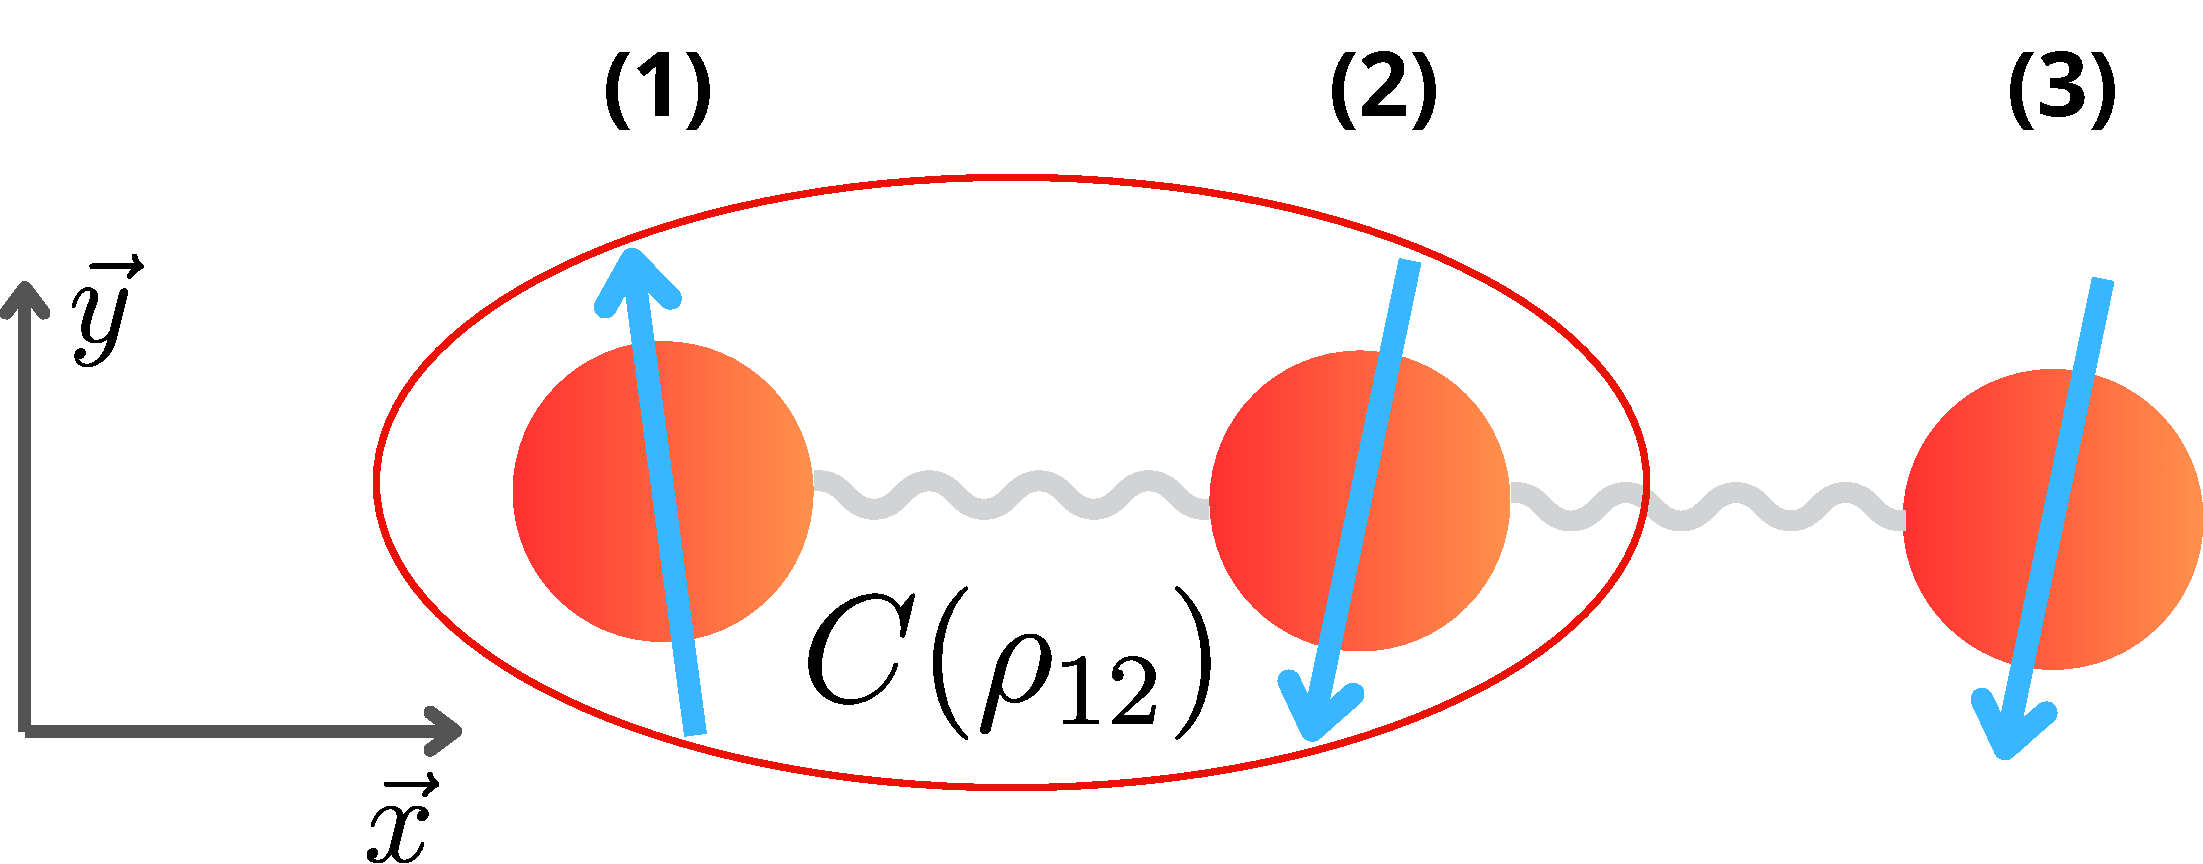
\includegraphics[width=\textwidth]{methodology/partial_trace_1.pdf}
        \caption{\centering Concurrence between the qubit (1) and (2)}
        \label{fig:Concurrence between the qubit (1) and (2)}
    \end{subfigure}
    \hfill
    \begin{subfigure}[b]{0.3\textwidth}
        \centering
        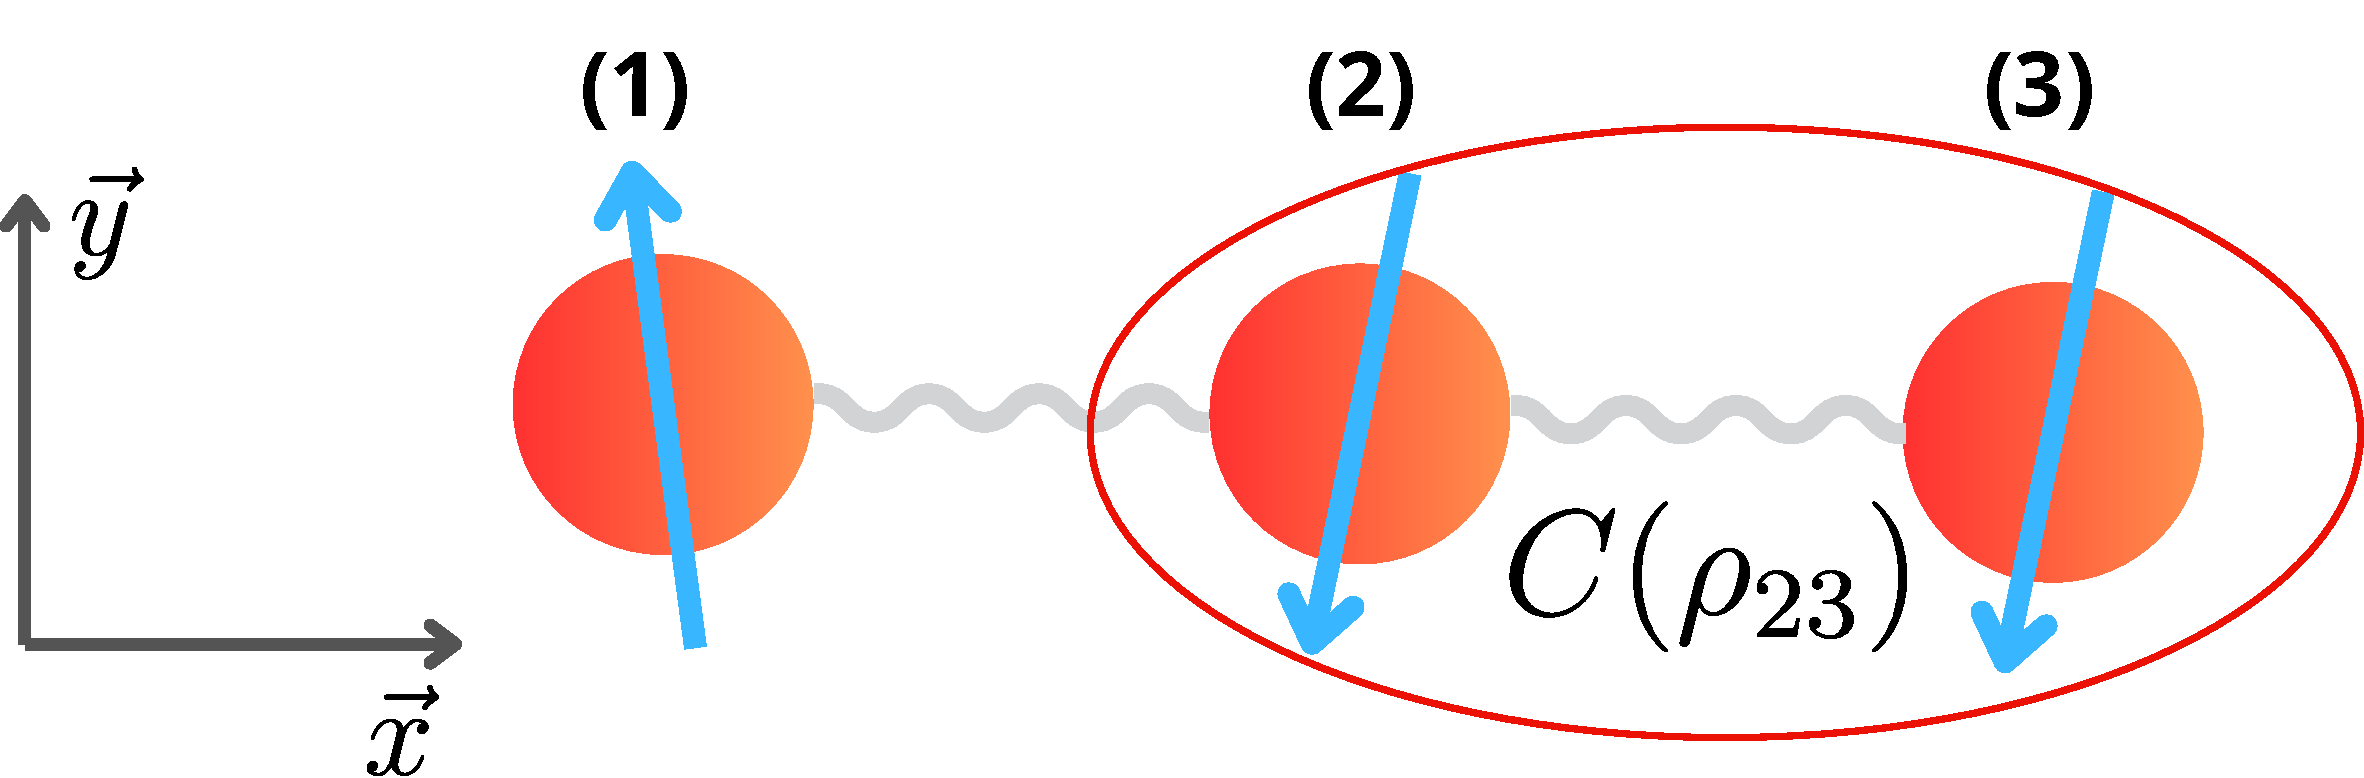
\includegraphics[width=\textwidth]{methodology/partial_trace_2.pdf}
        \caption{\centering Concurrence between the qubit (2) and (3)}
        \label{fig:Concurrence between the qubit (2) and (3)}
    \end{subfigure}
    \hfill
    \begin{subfigure}[b]{0.3\textwidth}
        \centering
        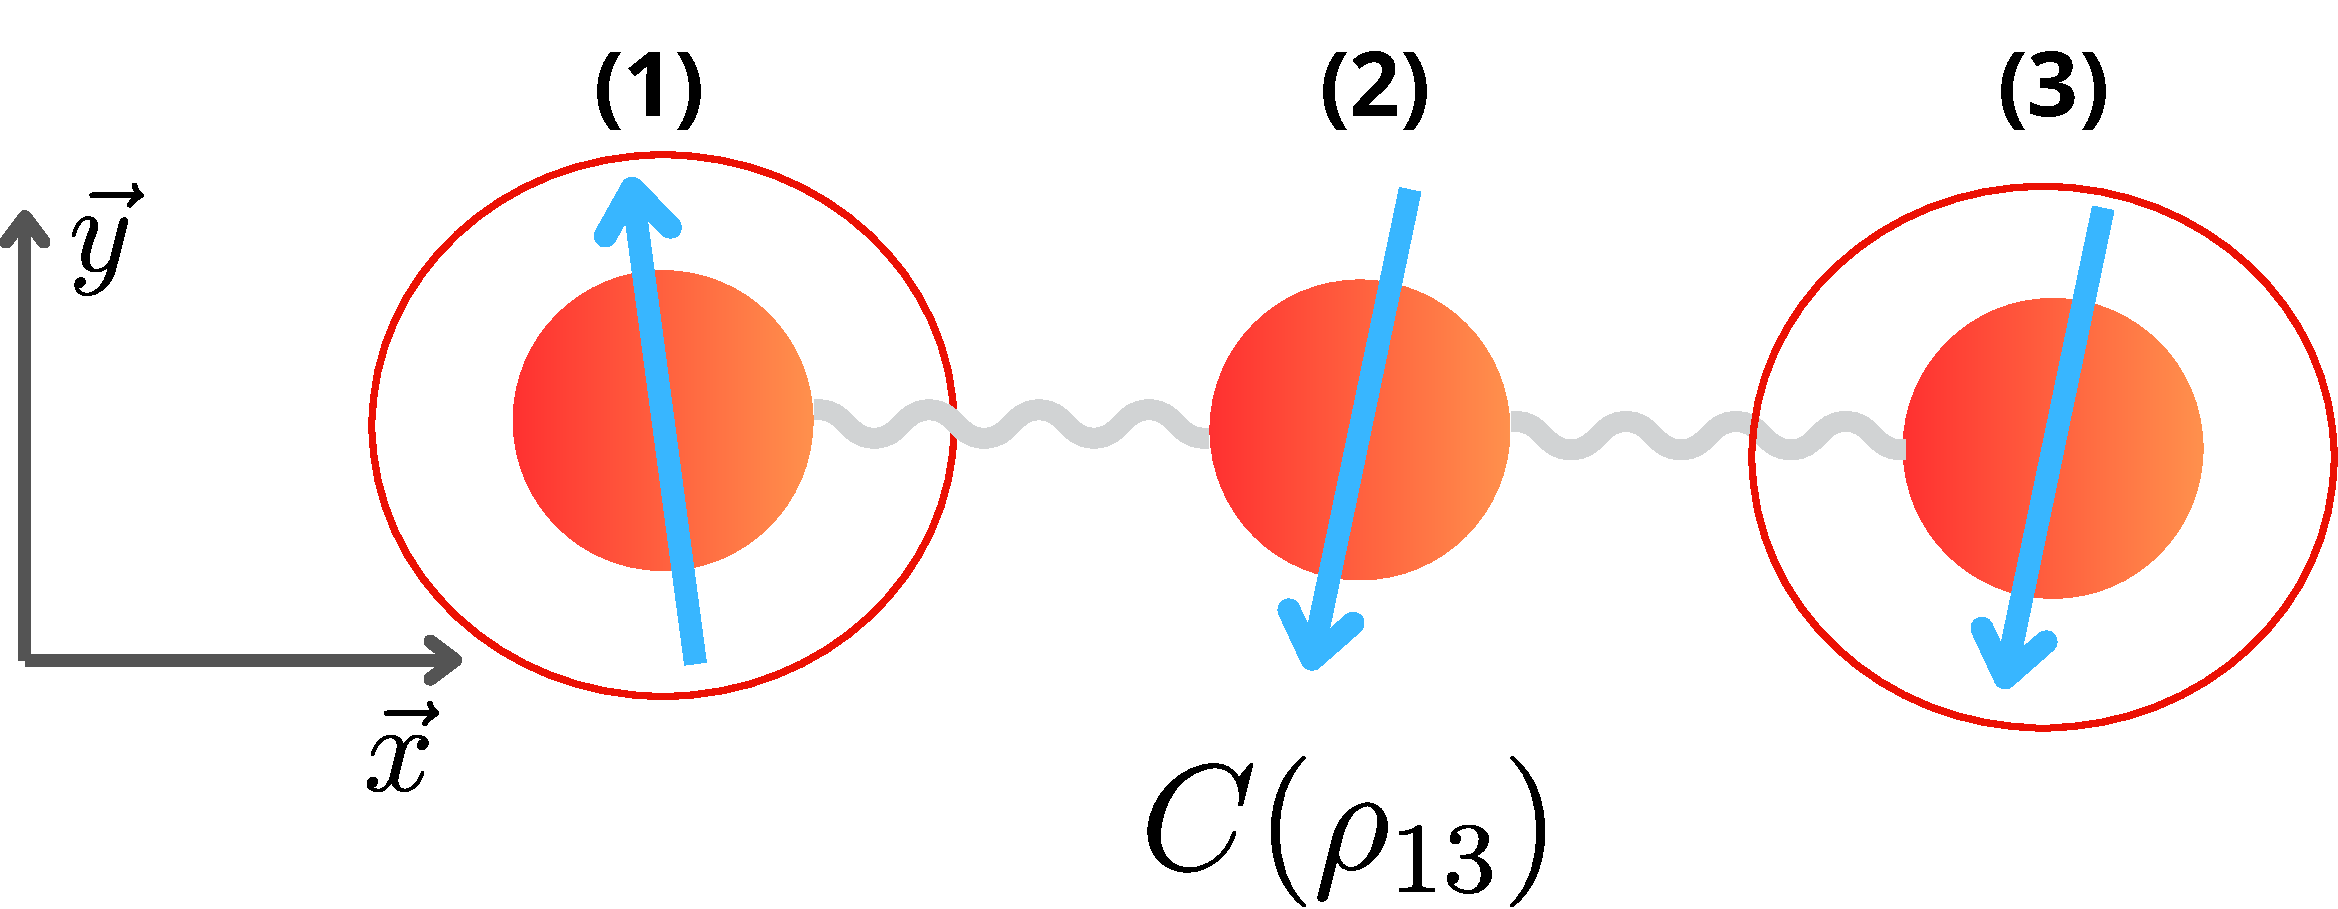
\includegraphics[width=\textwidth]{methodology/partial_trace_3.pdf}
        \caption{\centering Concurrence between the qubit (1) and (3)}
        \label{fig:Concurrence between the qubit (1) and (3)}
    \end{subfigure}
    \caption{Problem of calculation of the concurrence for many qubits}
    \label{fig:partial_traces}
\end{figure}



We understand we the \refig{fig:partial_traces} with have to a isolate the pair of the qubit and computed the density matrix of the 
couple of qubit note $\rho_{ij}$ where $i \neq j \text{ and } (i,j) \in \mathbb{N}^*$, for that we will use a mathematical tool call the partial
trace \cite{bradley_at_2020} 

\mydef{Partial trace}{
Let take a system of $L+1$ quantum system so 

\begin{equation}
    (i,j) \in (\mathbb{N}^*)^2 \text{ and } i \neq j , \ \rho_{ij} = \sumd{i=1}{\dim(A)} \bra*{e_i} \rho \ket{e_i}
\end{equation}

}{}

Let do a example
For example if we want to compute the density matrix of the system of the qubit (1) and (2) schematic 
in the \refig{fig:Concurrence between the qubit (1) and (2)} 








\newpage 

\section{Results And Discussion}


\subsection{Entanglement in a spin chain with 2 qubits}
In this section, we analyze the dynamics of a 
system consisting of two qubits with the Hamiltonian given by:

\[
    \hamil =  \hbar J\left [ \left ( \frac{1 + \delta}{2} \right ) \sigma_1^x \otimes 
    \sigma_2^x  + \left ( \frac{1 - \delta}{2} \right ) \sigma_1^y \otimes \sigma_2^y \right ] + 
    D \hbar \left ( \sigma_1^x \otimes \sigma_2^y + \gamma \sigma_1^y \otimes \sigma_2^x  \right ) + g \left( 
    \sigma_1^z \otimes \mathbb{\hat{I}} + \mathbb{\hat{I}} \otimes \sigma_2^z  
\right).
\]

we focus on the concurrence $C(\rho(t))$, which quantifies the entanglement between 
the two qubits. The analytical solution for the concurrence, as derived in Appendix B, is given by:

\begin{equation*}
        C(\rho(t)) = \abs*{\sin(2 \mu t)},
\end{equation*}

where \(\mu = \sqrt{J^2 + D^2(\gamma-1)^2}\).

We plot the concurrence in the figure 


We can see the plot of $C(\ket{\psi (t)})$ for the $\ket{\psi (t)}$ at \myeqref{eq: psi t} in the figure 

    \begin{figure}[h!]
        \centering
        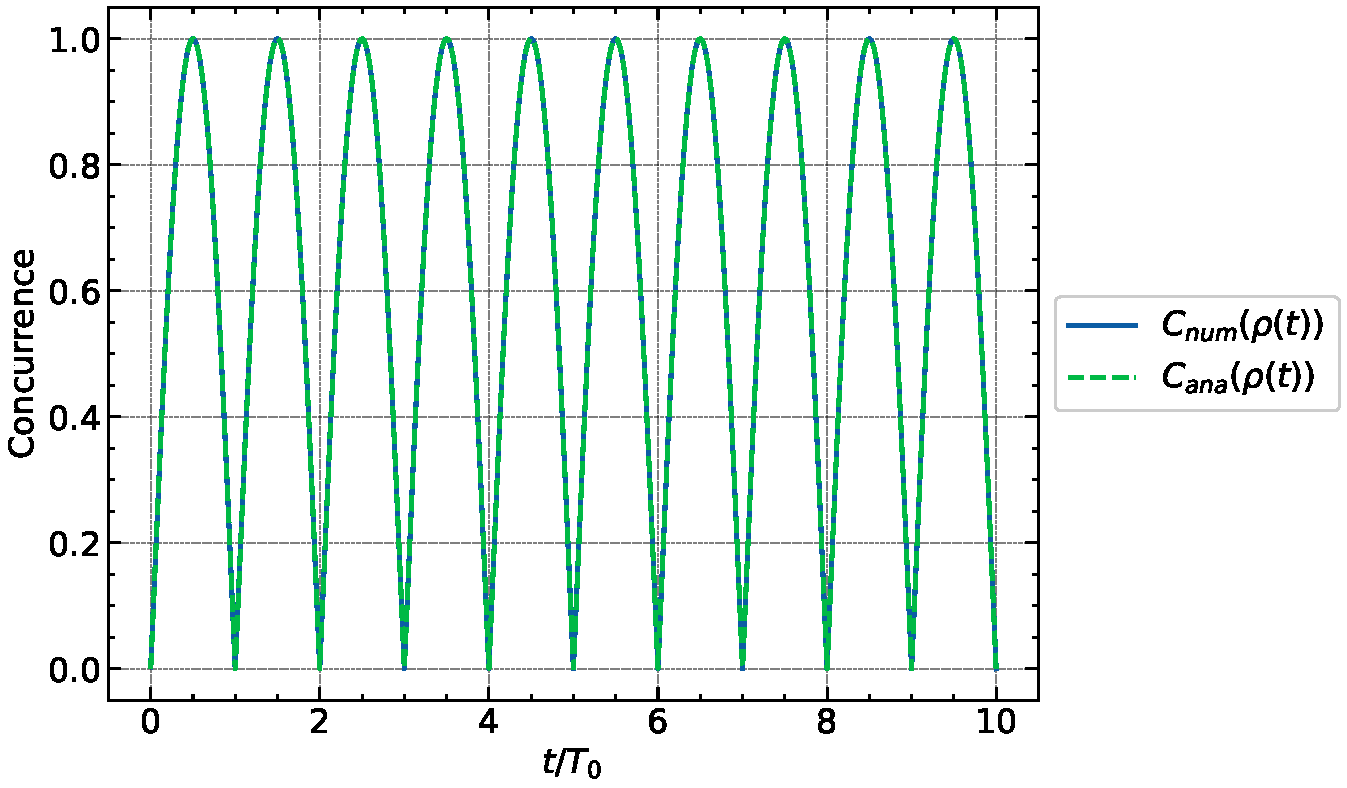
\includegraphics[width=0.8\linewidth]{results_and_discussion/2_qubits/up_down_with_ana_0.pdf}
        \caption{\centering $D=0$, Mean Squared Error: 1.51e-07, $\gamma = -1$, $\delta = 1$, $g = 1$, $J = 1$}
        \label{fig:concurrencecpsiD_0}
    \end{figure}
    \begin{figure}[h!]
        \centering
        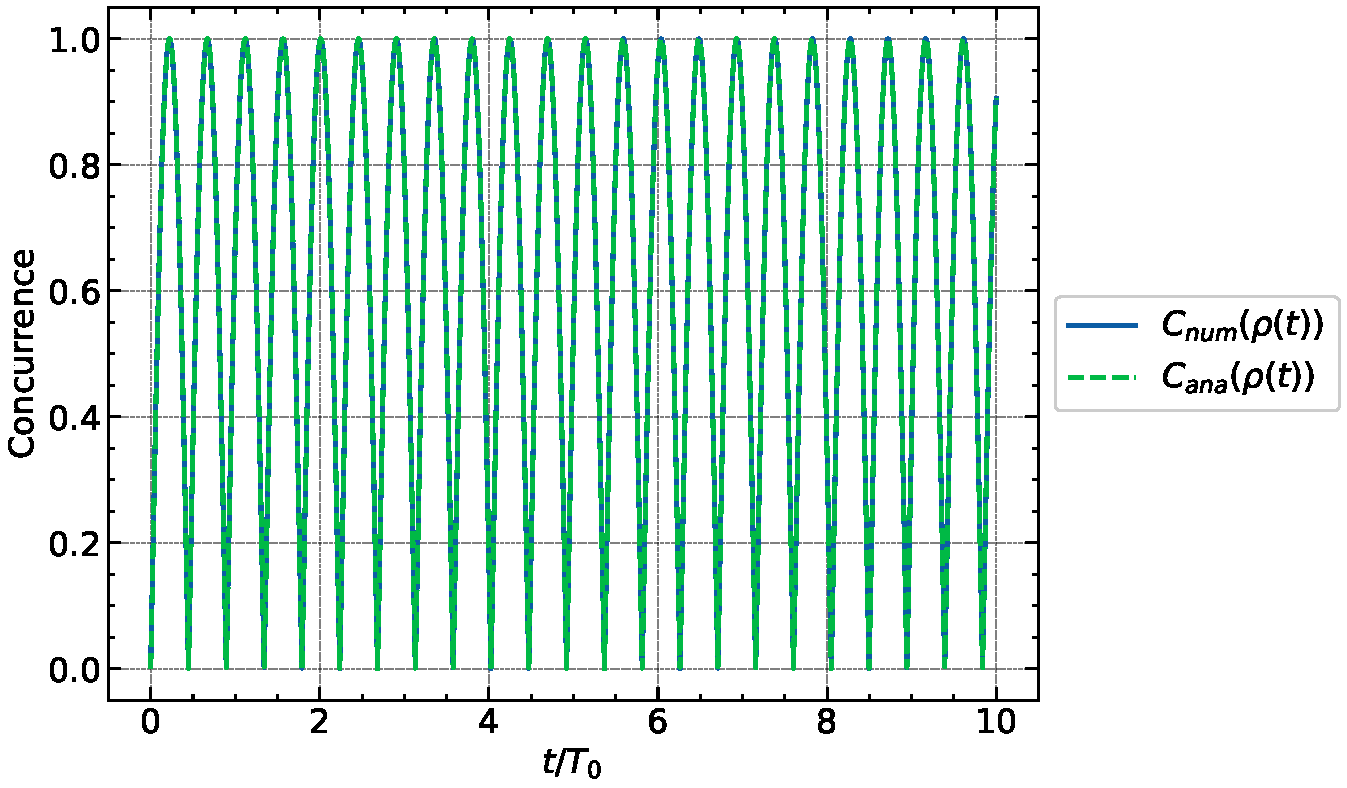
\includegraphics[width=0.8\linewidth]{results_and_discussion/2_qubits/up_down_with_ana_1.pdf}
        \caption{\centering $D=1$, Mean Squared Error: 1.51e-07, $\gamma = -1$, $\delta = 1$, $g = 1$, $J = 1$}
        \label{fig:concurrencecpsiD_1}
    \end{figure}

\newpage

The concurrence formula reveals a simple yet profound oscillatory behavior of the entanglement between the qubits. The parameter \(\mu\) plays a crucial role in determining the frequency of these oscillations, which depends on the coupling constants \(J\) and \(D\) as well as the anisotropy parameter \(\gamma\).

\textbf{Impact of Coupling Constants \(J\) and \(D\):}

The coupling constant \(J\) directly contributes to \(\mu\), indicating that a stronger XX and YY interaction 
        leads to faster oscillations in concurrence. The term \(D(\gamma-1)\) suggests 
        that the effect of the \(D\) coupling on the concurrence 
        is modulated by the anisotropy \(\gamma\). For \(\gamma = 1\), 
        this contribution vanishes, and the oscillation frequency is 
        solely determined by \(J\). However, for \(\gamma \neq 1\), 
        the anisotropy introduces additional dynamics through \(D\).


 \textbf{Behavior for Different Regimes of \(\mu\):}

 When \(\mu\) is large (e.g., large \(J\) 
        or significant anisotropy), the concurrence oscillates 
        rapidly, meaning that the system frequently transitions 
        between entangled and separable states. For small \(\mu\), the oscillations are slower, 
        indicating more prolonged periods of either high or low entanglement.

\textbf{Maximal Concurrence:}
 The concurrence achieves its maximum value of 1 when \(\sin(2 \mu t) = \pm 1\), indicating a fully entangled state.
 Conversely, \(C(\ket*{\psi(t)}) = 0\) when \(\sin(2 \mu t) = 0\), representing separable states where the qubits are not entangled.

\subsection{Discussion}

The results provide significant insights into the entanglement 
dynamics in a two-qubit system with anisotropic and cross-coupling terms. 
The oscillatory nature of the concurrence reflects the intricate interplay 
between different types of interactions present in the Hamiltonian. 
This behavior is essential for applications in quantum information 
processing, where control over entanglement is crucial.

\begin{itemize}
    \item \textbf{Quantum Control:} By tuning the parameters 
    \(J\), \(D\), and \(\gamma\), one can manipulate 
    the entanglement dynamics, potentially allowing for 
    the design of specific quantum gates or the 
    implementation of quantum error correction protocols that rely on dynamic entanglement.

    \item \textbf{Effect of Anisotropy:} The dependence of \(\mu\) on 
    \(\gamma\) illustrates how anisotropy can either enhance or diminish 
    the contribution of the \(D\) coupling to the entanglement dynamics. 
    This result suggests that systems with tunable anisotropy could be 
    particularly versatile in quantum control schemes.

    \item \textbf{Robustness of Entanglement:} The periodic nature of the concurrence indicates that, under specific conditions, entanglement can be robust over time, recurring predictably as a function of time. This property might be exploited to maintain entanglement over long durations in quantum communication protocols.
\end{itemize}

In Conclusion
 concurrence 
 quantifies the entanglement between two qubits. 
 For example, when \(t/T_0 = 0.5 + k\), where \(k \in \mathbb{N}\), the concurrence is 1. At this time, the state \(\ket{\psi (t)}\) is:


 
 \begin{equation*}
 	\ket{\psi \left( t = \frac{\pi}{4} + \frac{k\pi}{2}\right) } = \frac{1}{\sqrt{2}} \ket{\uparrow \downarrow} - \frac{i(J + iD(\gamma -1))}{\sqrt{2}\gamma}   \ket{\downarrow \uparrow}
 \end{equation*}
 
 
This state is evidently entangled according to the definition.

Moreover we can recognize a Bell state we this form: 

\begin{equation}
		\ket{\psi \left( t = \frac{\pi}{4} + \frac{k\pi}{2}\right) } = \frac{1}{\sqrt{2}} \left(  \ket{\uparrow \downarrow} -ie^{i\theta}\ket{\uparrow \downarrow}  \right)
\end{equation}

where $ \theta = \arctan\left( \frac{D(\gamma -1)}{J}\right)$


 
And at $t/T_0 = k$ the concurrence equal to $0$, 

 \begin{equation*}
	\ket{\psi \left( t = \frac{k\pi}{2}\right) } = \frac{i(J + iD(\gamma -1))}{\sqrt{2}\gamma}   \ket{\downarrow \uparrow}
\end{equation*}

In this case, the state is separable.
	

\newpage
\subsection{Entanglement in a spin chain with N qubits}
This study systematically investigates the concurrence in a three-qubit system and a six-qubit system
governed by the Heisenberg XY model, incorporating the Dzyaloshinskii-Moriya interaction (DMI). 
The primary parameters analyzed include the DMI constant \(D\), the anisotropy parameter \(\delta\), and the correction factor 
\(\gamma\). The concurrence between pairs of qubits was assessed under various configurations of these parameters.


\subsubsection{Entanglement in a spin chain with 3 qubits}


The concurrence values varied from 0.0 to approximately 0.8, indicating robust entanglement within the qubit system. 
The pairwise concurrences \( (C_{1,2}, C_{1,3}, C_{2,3}) \) exhibited a consistent pattern, with entanglement gradually 
diminishing over time.

In the first subfigure \refig{fig:subfig1}, the concurrence values show a peak of approximately 0.8 with \( D = 0 \), \( \gamma = 1 \), and \( \delta = 0 \). With an increase in the anisotropy parameter to \( \delta = 1 \) \refig{fig:subfig2}, 
the concurrence values remained relatively high, albeit slightly lower than in the previous case. The maximum concurrence observed 
was around 0.6, with a similar temporal decline in entanglement distribution across the qubits.

The introduction of DMI with \( D = 1 \) \refig{fig:subfig3} resulted in a slight enhancement of concurrence values, reaching a peak of 
approximately 0.8. This suggests that DMI strengthens the entanglement between qubits, with the pairwise concurrences following a similar pattern 
to earlier configurations but with marginally higher values.

When both \( D \) and \( \delta \) were set to 1 \refig{fig:subfig4}, the concurrence values were slightly lower, 
peaking at about 0.6. The entanglement distribution remained similar across qubit pairs, 
though the overall entanglement was reduced compared to 
the scenario with \( D = 1 \) and \( \delta = 0 \).

\begin{figure}[h!]
    \centering
    \begin{subfigure}[b]{0.48\textwidth}
        \centering
        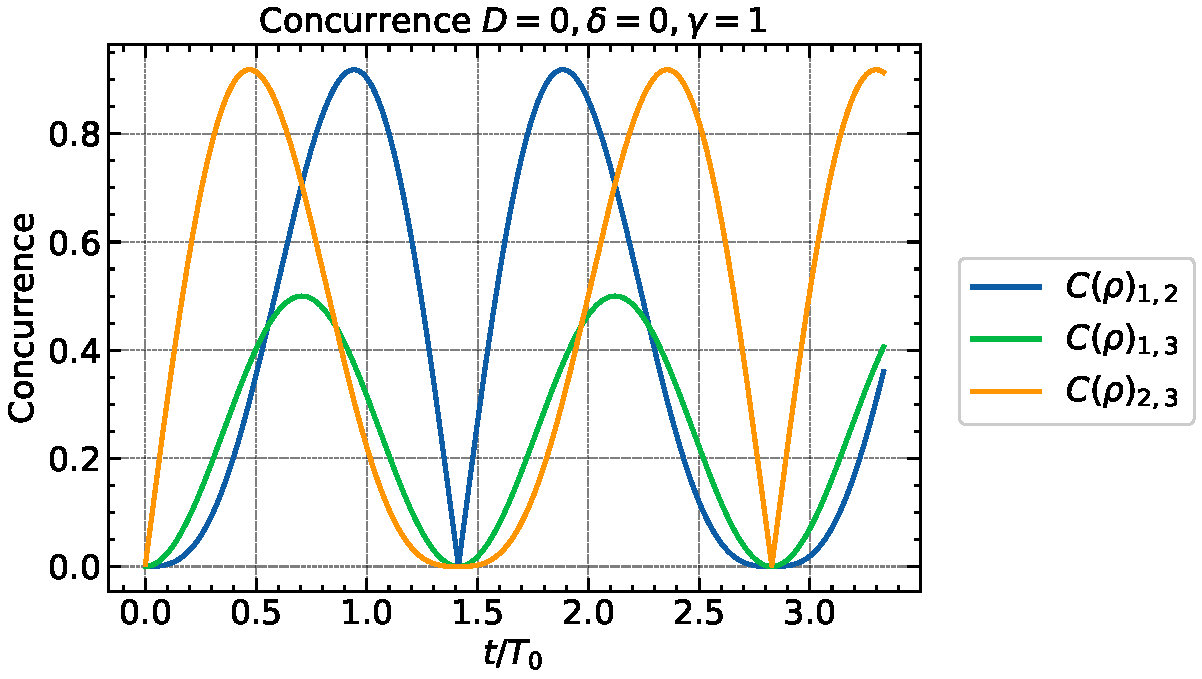
\includegraphics[width=\linewidth]{results_and_discussion/3_qubits/up_down_with_ana_0_1_0.pdf}
        \caption{Concurrence for \( D = 0\), \( \gamma = 1\), \( \delta = 0\)}
        \label{fig:subfig1}
    \end{subfigure}
    \hfill
    \begin{subfigure}[b]{0.48\textwidth}
        \centering
        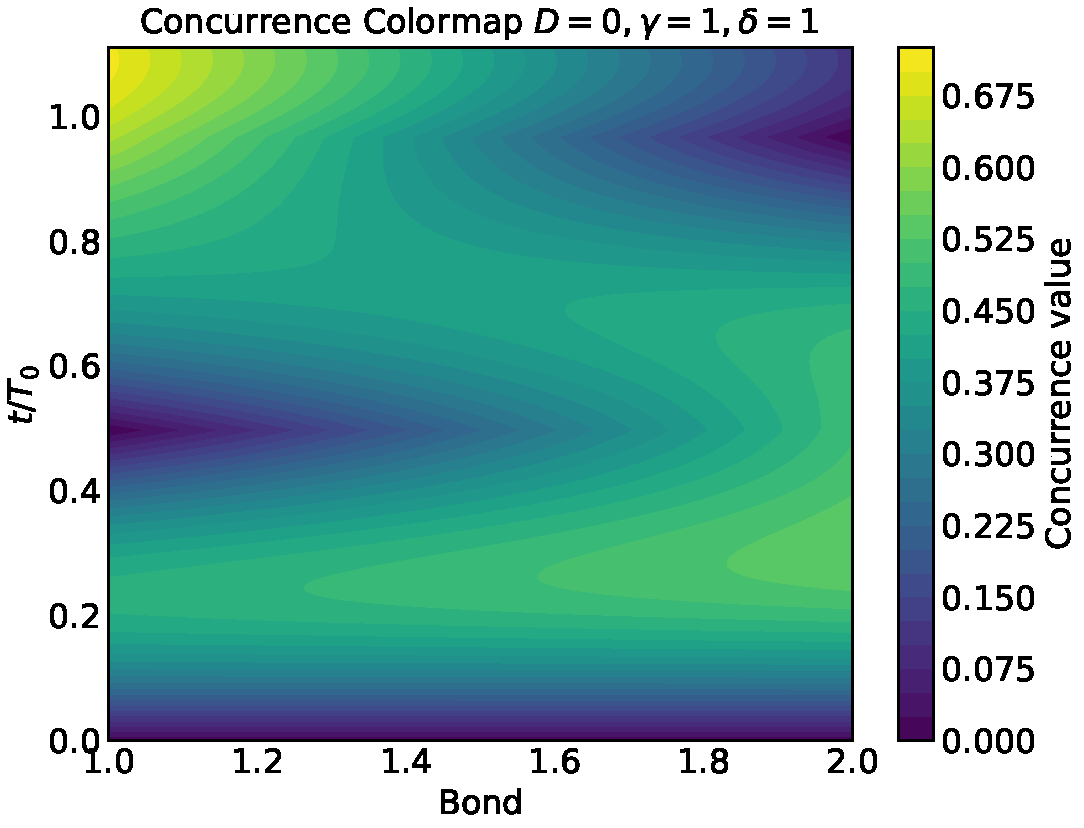
\includegraphics[width=\linewidth]{results_and_discussion/3_qubits/up_down_with_ana_0_1_1.pdf}
        \caption{Concurrence for \( D = 0\), \( \gamma = 1\), \( \delta = 1\)}
        \label{fig:subfig2}
    \end{subfigure}

    \vspace{0.5cm}

    \begin{subfigure}[b]{0.48\textwidth}
        \centering
        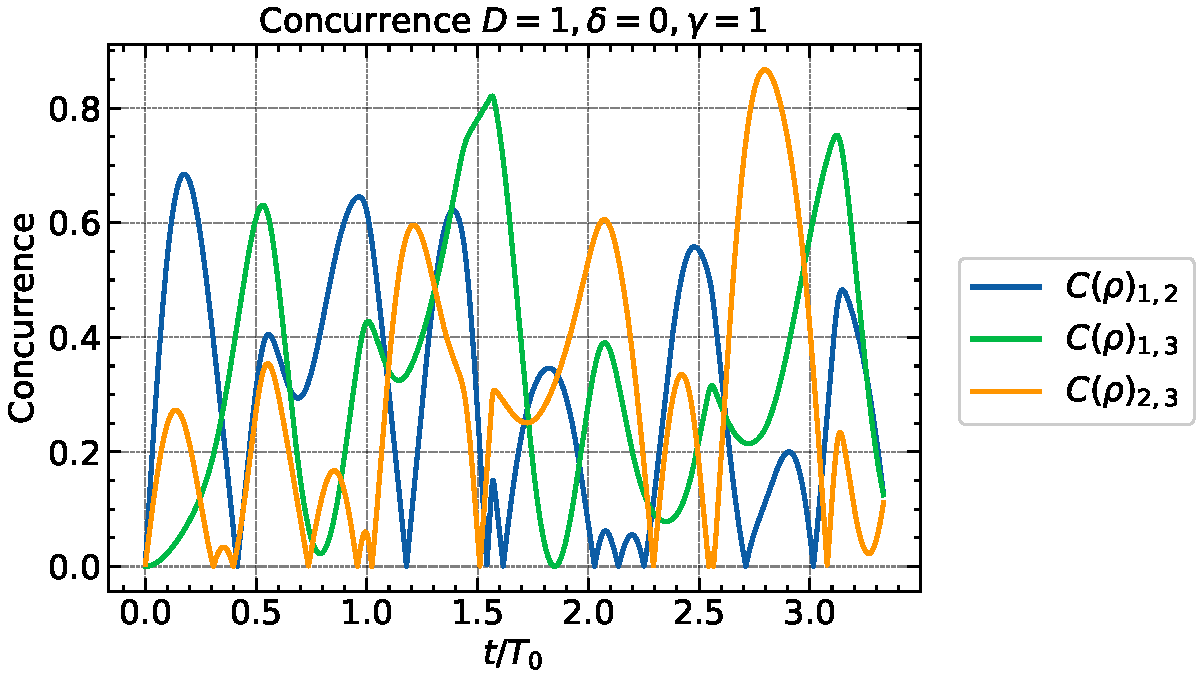
\includegraphics[width=\linewidth]{results_and_discussion/3_qubits/up_down_with_ana_1_1_0.pdf}
        \caption{Concurrence for \( D = 1\), \( \gamma = 1\), \( \delta = 0\)}
        \label{fig:subfig3}
    \end{subfigure}
    \hfill
    \begin{subfigure}[b]{0.48\textwidth}
        \centering
        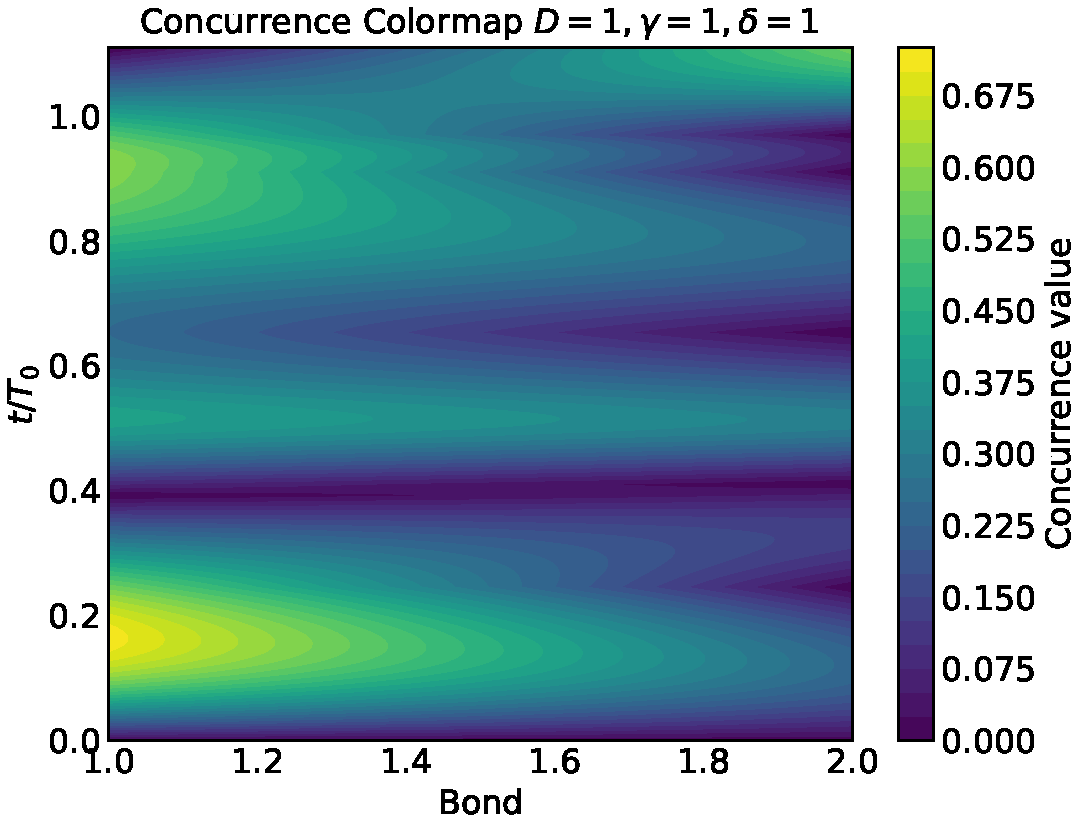
\includegraphics[width=\linewidth]{results_and_discussion/3_qubits/up_down_with_ana_1_1_1.pdf}
        \caption{Concurrence for \( D = 1\), \( \gamma = 1\), \( \delta = 1\)}
        \label{fig:subfig4}
    \end{subfigure}

    \caption{Concurrence for different values of \( D \) and \( \delta \) with \( \gamma = 1 \). The concurrence values indicate the level of entanglement in the qubit system over time, showing how different parameters influence the entanglement.}
    \label{fig:concurrence_comparison}
\end{figure}


\newpage
\textbf{Discussion}

The findings highlight the significant role of the Dzyaloshinskii-Moriya interaction in influencing the entanglement characteristics of the three-qubit system. The DMI, quantified by \(D\), generally enhances concurrence, indicating stronger entanglement. This effect is particularly pronounced when comparing scenarios with \(D = 0\) and \(D = 1\).

Conversely, the anisotropy parameter \(\delta\) introduces a competing influence that can diminish the overall entanglement as it increases. Specifically, when \(\delta = 1\), the system exhibits lower concurrence values compared to \(\delta = 0\), even in the presence of DMI. This suggests that while DMI tends to enhance entanglement, increasing \(\delta\) may counteract this effect, possibly due to modifications in the system's symmetry or interaction strengths.

In the absence of DMI (\(D = 0\)), the system still demonstrates significant entanglement, especially when \(\gamma = 1\) and \(\delta = 0\), with concurrence values reaching up to 0.8. This indicates that the Heisenberg XY model inherently supports strong entanglement, which can be modulated by adjusting the DMI and anisotropy parameters.




\newpage
\subsubsection{Entanglement in a spin chain with 6 qubits}
\textbf{Concurrence for \( D = 0, \gamma = 1, \delta = 0 \):} \refig{fig:6q_0_1_0}
The concurrence values in this configuration range from 0.00 to approximately 0.81, showing a high level of entanglement that gradually decreases as the system evolves over time. The colormap indicates a relatively uniform distribution of entanglement across the bonds in the lattice.


\textbf{Concurrence for \( D = 0, \gamma = 1, \delta = 1 \):} \refig{fig:6q_0_1_1}
When \(\delta\) is increased to 1, the maximum concurrence value decreases slightly to approximately 0.675. The distribution of concurrence values remains similar to the previous case, with the entanglement decreasing over time, but with a slightly reduced maximum entanglement value.


\textbf{Concurrence for \( D = 1, \gamma = 1, \delta = 0 \):} \refig{fig:6q_0_1_0}
Introducing the DMI constant \(D = 1\) while keeping \(\gamma = 1\) and \(\delta = 0\) leads to an increase in the maximum concurrence value to around 0.81. This increase suggests that the DMI enhances the entanglement within the system. The distribution of concurrence is still fairly uniform across the lattice, indicating that the DMI positively influences the overall entanglement.


\textbf{Concurrence for \( D = 1, \gamma = 1, \delta = 1 \):} \refig{fig:6q_1_1_1}
When both \(D\) and \(\delta\) are set to 1, the system exhibits a maximum concurrence value of approximately 0.56, 
which is lower than when \(\delta = 0\). This suggests that while the DMI increases entanglement, the anisotropy 
parameter \(\delta\) introduces an effect that reduces the overall entanglement when \(\gamma\) is also present.
\begin{figure}[h!]
    \centering
    \begin{subfigure}[b]{0.48\textwidth}
        \centering
        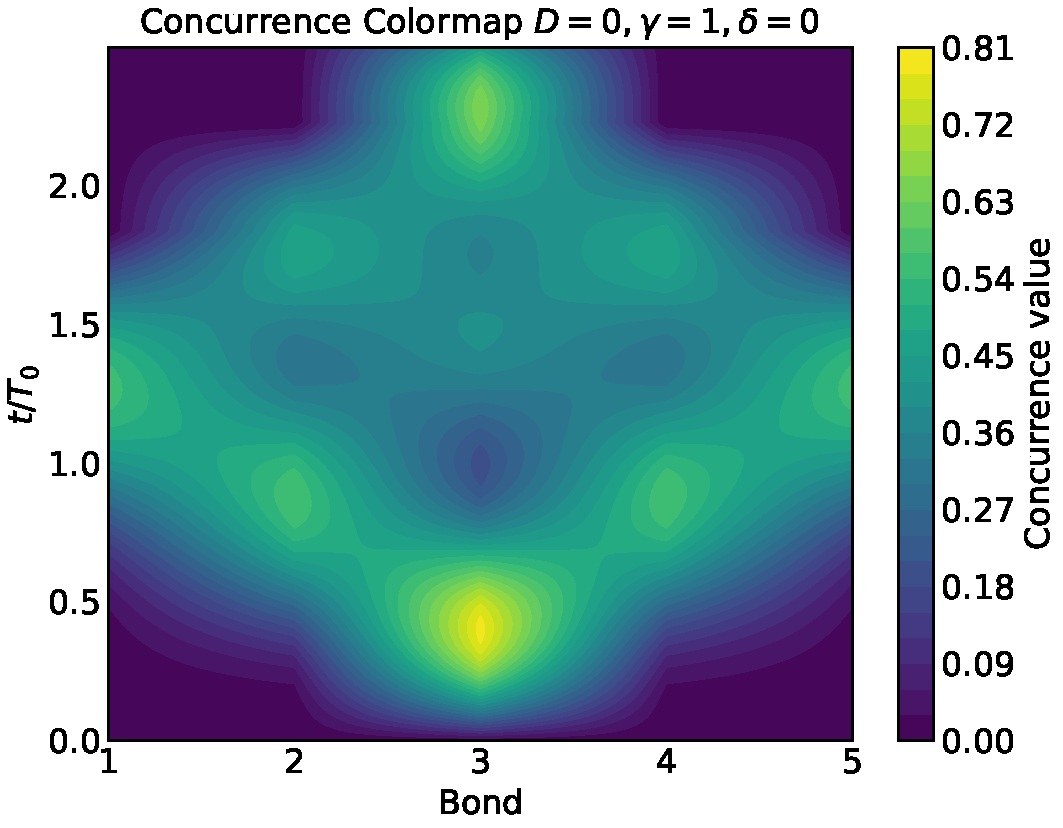
\includegraphics[width=\linewidth]{results_and_discussion/6_qubits/up_down_with_ana_0_1_0.pdf}
        \caption{Concurrence for \( D = 0, \gamma = 1, \delta = 0 \)}
        \label{fig:6q_0_1_0}
    \end{subfigure}
    \hfill
    \begin{subfigure}[b]{0.48\textwidth}
        \centering
        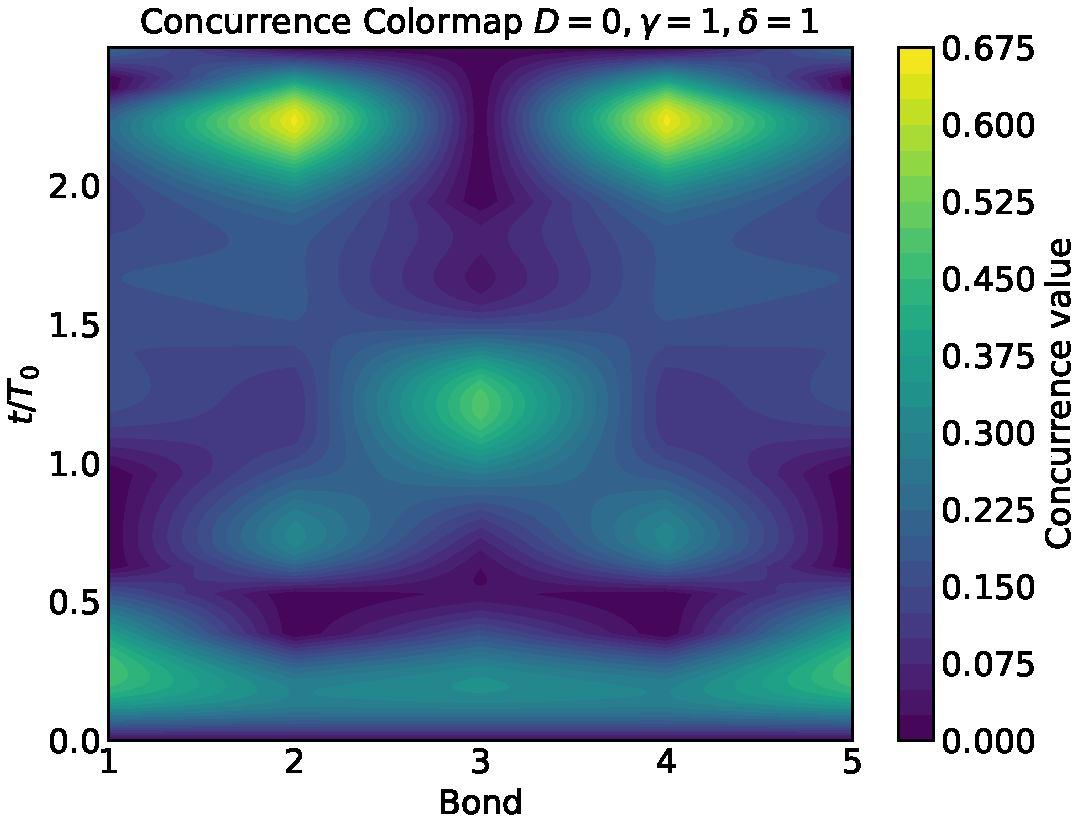
\includegraphics[width=\linewidth]{results_and_discussion/6_qubits/up_down_with_ana_0_1_1.pdf}
        \caption{Concurrence for \( D = 0, \gamma = 1, \delta = 1 \)}
        \label{fig:6q_0_1_1}
    \end{subfigure}

    \vspace{0.5cm}

    \begin{subfigure}[b]{0.48\textwidth}
        \centering
        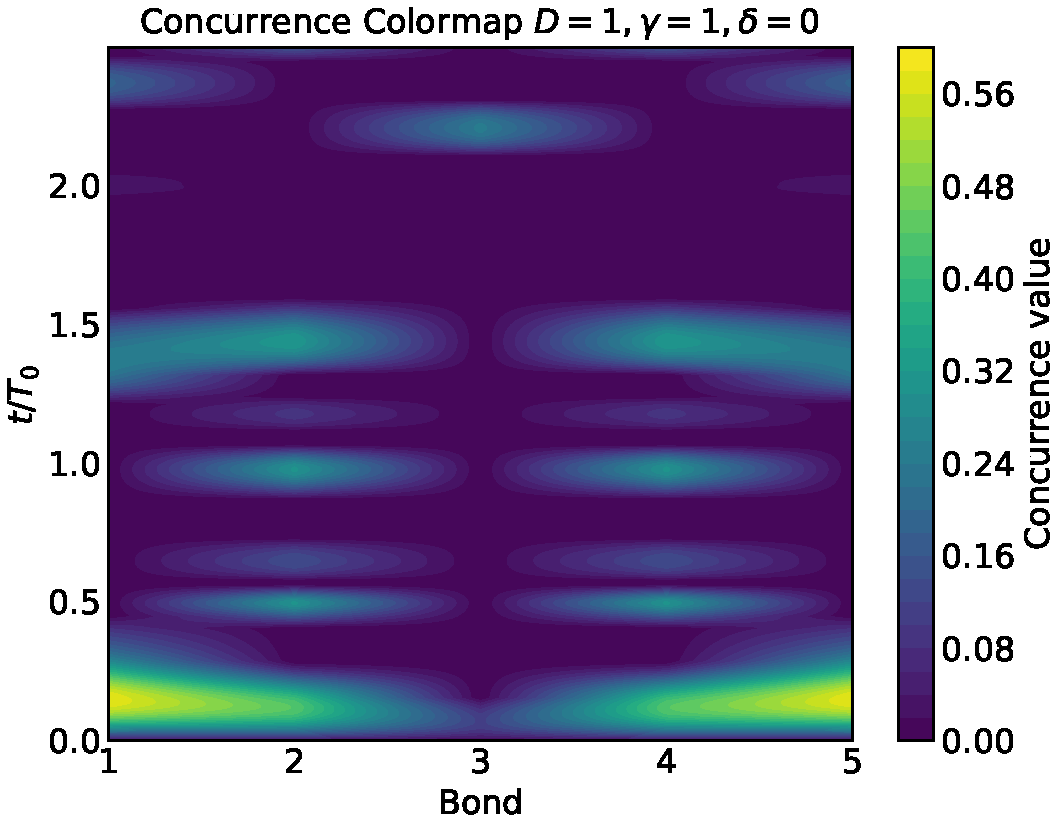
\includegraphics[width=\linewidth]{results_and_discussion/6_qubits/up_down_with_ana_1_1_0.pdf}
        \caption{Concurrence for \( D = 1, \gamma = 1, \delta = 0 \)}
        \label{fig:6q_1_1_0}
    \end{subfigure}
    \hfill
    \begin{subfigure}[b]{0.48\textwidth}
        \centering
        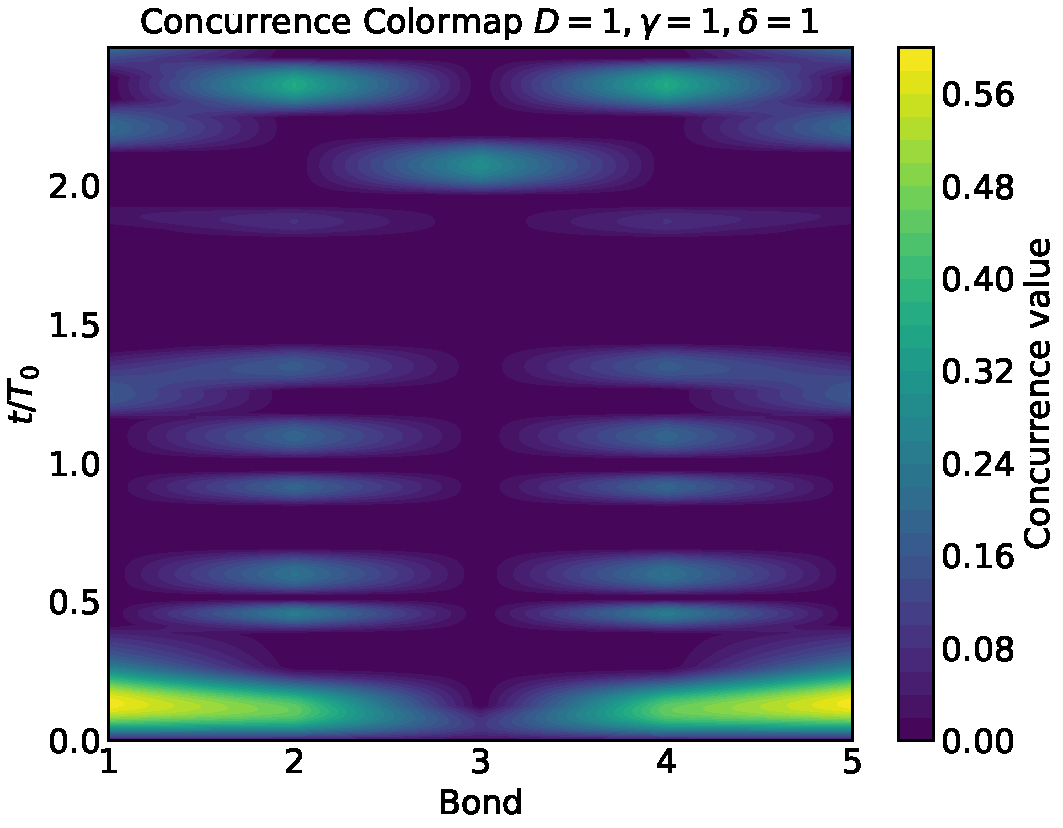
\includegraphics[width=\linewidth]{results_and_discussion/6_qubits/up_down_with_ana_1_1_1.pdf}
        \caption{Concurrence for \( D = 1, \gamma = 1, \delta = 1 \)}
        \label{fig:6q_1_1_1}
    \end{subfigure}

    \caption{Concurrence for different values of \( D \) and \( \delta \) with \( \gamma = 1 \) in a 6-qubit system. The plots illustrate how these parameters affect the entanglement within the system over time.}
    \label{fig:concurrence_comparison_6qubits}
\end{figure}





The results indicate that the Dzyaloshinskii-Moriya interaction (DMI) significantly influences the entanglement properties of the 
system. Specifically, the concurrence values increase when the DMI constant \(D\) is set to 1, implying that the DMI fosters 
stronger entanglement between the qubits in the lattice. This enhancement is evident when comparing cases with \(D = 0\) and 
\(D = 1\), where the latter consistently shows higher concurrence values.

However, the anisotropy parameter \(\delta\) and the correction factor \(\gamma\) introduce competing effects. When 
\(\delta = 1\) and \(\gamma = 1\), the concurrence is lower compared to when \(\delta = 0\) and \(\gamma = 1\), even 
in the presence of DMI. This reduction suggests that the anisotropy, along with \(\gamma\), can counteract the positive 
impact of DMI on entanglement. The interplay between these parameters likely alters the symmetry and interaction strength
within the lattice, thereby influencing the entanglement.

In scenarios where \(D = 0\), the system still exhibits significant entanglement, particularly when 
\(\gamma = 1\) and \(\delta = 0\), with concurrence values reaching up to approximately 0.81. 
This demonstrates that the Heisenberg XY model itself supports strong entanglement, but this can be 
modulated by the presence of DMI and adjustments to \(\delta\) and \(\gamma\).






\newpage

\section*{Conclusion}
\addcontentsline{toc}{section}{Conclusion}
This study provides a comprehensive 
analysis of the entanglement properties 
in both 2-qubit, 3-qubit and 6-qubit systems modeled 
by the Heisenberg XY Hamiltonian with 
Dzyaloshinskii-Moriya interaction (DMI). 
The key findings from our analysis 
can be summarized as follows:

\begin{enumerate}
    \item \textbf{Impact of Dzyaloshinskii-Moriya Interaction (DMI):}
    The presence of the DMI, represented by the parameter \(D\), consistently enhances the entanglement between qubits. This is observed through increased concurrence values in both the 2-qubit, 3-qubit and 
    6-qubit systems when \(D = 1\) compared to when \(D = 0\). The DMI facilitates stronger quantum correlations, making it a valuable tool for increasing entanglement in quantum systems.

    \item \textbf{Effect of Anisotropy Parameter \(\delta\):}
    The anisotropy parameter \(\delta\) introduces a counteracting influence on the entanglement. While the system shows high concurrence values when \(\delta = 0\), an increase in \(\delta\) generally leads to a reduction in these values, especially in the presence of DMI. This suggests that \(\delta\) affects the symmetry and interaction strengths within the lattice, reducing the overall entanglement when increased.

\end{enumerate}

In conclusion, the Dzyaloshinskii-Moriya interaction 
and the anisotropy parameter provide powerful 
mechanisms for manipulating entanglement in 
quantum systems. Understanding how these parameters 
influence entanglement allows for the precise control of the 
quantum system, which has significant implications for the development of quantum technologies. 
This study lays the groundwork 
for future research into optimizing 
entanglement in more complex quantum systems and exploring the practical applications of these findings in 
quantum computing and materials science.
\newpage 

\bibliographystyle{plain}
\bibliography{Intership_USACH.bib}

\newpage 


\pagestyle{romanstyle_2}
\pagenumbering{roman}

\appendix
\appendixpage

\startcontents[sections]
\printcontents[sections]{l}{1}{\setcounter{tocdepth}{2}}

\section{Appendix First}
\subsection{Generalities and Recall on Matrix Series}


\mydef{Norme matrix}{For \( A = (a_{ij}) \in M_n(\mathbb{C}) \), we define
	\[ \|A\|_\infty = \max \{|a_{ij}| ; 1 \leq i, j \leq n\}. \]
	
	\(\|\cdot\|_\infty\) is a norm on \( M_n(\mathbb{C}) \), i.e., it is a function with values in \( \mathbb{R}^+ \) such that
	\begin{itemize}
		\item \( \forall A, \|A\|_\infty = 0 \iff A = 0 \),
		\item \( \forall A, \forall \lambda \in \mathbb{C}, \|\lambda A\|_\infty = |\lambda| \cdot \|A\|_\infty \),
		\item \( \forall A, B, \|A + B\|_\infty \leq \|A\|_\infty + \|B\|_\infty \).
	\end{itemize}
	

	
	
	}{Norme matrix}

In the following, we will denote \( \|\cdot\| \) instead of \( \|\cdot\|_\infty \).


\mydef{Converge sequence of matrix}{


\begin{itemize}
	\item A sequence \( (A_k) \) of \( M_n(\mathbb{C}) \) is said to be convergent if there exists \( A \in M_n(\mathbb{C}) \) such that \( \forall \epsilon > 0, \exists k_0 \in \mathbb{N} \) such that \( k \geq k_0 \Rightarrow \|A_k - A\| < \epsilon \).
	\item A sequence \( (A_k) \) is said to be Cauchy if \( \forall \epsilon > 0, \exists k_0 \in \mathbb{N}, \forall k, k_0 \geq k_0, \|A_k - A_{k_0}\| < \epsilon \).
\end{itemize}

}{Converge sequence of matrix}


\myprop{Characterization of matrix convergence}{Let \( (A_k) \) be a 
sequence of \( M_n(\mathbb{C}) \). Then it is Cauchy if and only if it is convergent.}{Characterization of matrix convergence}


\begin{proof}
	The right-to-left direction is classical, and the direct direction relies on the completeness of \( \mathbb{C} \)
\end{proof}


\mydef{Convergent and Absolutely convergent matrix serie}{Given a sequence \( (A_k) \) of \( M_n(\mathbb{C}) \), we define the associated series denoted \( \sum A_k \) as the sequence \( (S_k) \) with general term
	\[ S_k = \sum_{l=0}^{k} A_l. \]

The series is said to be absolutely convergent if the real series \( \sum \|A_k\| \) is convergent.}{Convergent 
and Absolutely convergent matrix serie}




\myprop{Convergent and Absolutely convergent matrix serie}{If \( \sum A_k \) is absolutely convergent, then it is convergent.}
{Convergent and Absolutely convergent matrix serie}


\begin{proof}
	Let \( \epsilon > 0 \). For all \( k \in \mathbb{N} \), denote \( T_k = \sum_{l=0}^{k} \|A_l\| \) and \( S_k = \sum_{l=0}^{k} A_l \). By hypothesis, \( (T_k) \) converges (in \( \mathbb{R} \)), so it is Cauchy. Hence, there exists \( k_0 \in \mathbb{N} \) such that for \( k, k_0 \geq k_0 \), we have \( |T_k - T_{k_0}| < \epsilon \).
	
	For \( k_0 \geq k \geq k_0 \), we have
	\[ \|S_{k_0} - S_k\| = \left\| \sum_{l=k+1}^{k_0} A_l \right\| \leq \sum_{l=k+1}^{k_0} \|A_l\| = T_{k_0} - T_k < \epsilon. \]
	Thus, the sequence \( (S_k) \) is Cauchy, hence convergent.
\end{proof}



\mylemma{Matrix inequality}{For \( A, B \in M_n(\mathbb{C}) \),
	\[ \|AB\| \leq n \|A\| \|B\| \quad \text{and} \quad \|A^k\| \leq n^{k-1} \|A\|^k. \]}{Matrix inequality}


\begin{proof}
Let \( A = (a_{ij}), B = (b_{ij}), \) and \( C = AB = (c_{ij}) \). For all \( i, j \),
\[ |c_{ij}| = \left| \sum_{k=1}^{n} a_{ik} b_{kj} \right| \leq \sum_{k=1}^{n} |a_{ik}||b_{kj}| \leq \sum_{k=1}^{n} \|A\| \|B\| = n \|A\| \|B\|. \]
Consequently, \( \|C\| \leq n \|A\| \|B\| \).

The second inequality is obtained by induction on \( k \) using the first.
\end{proof}





	
\subsection{Properties exponential of matrix}
	
\mydef{Exponential of matrix}{Let \( A \in M_n(\mathbb{C}) \). We define \( e^A = \exp(A) \in M_n(\mathbb{C}) \) by
	\[ e^A = \sum_{k=0}^{+\infty} \frac{A^k}{k!}. \]}{Properties exponential of matrix}
	

\myth{Existance of the exponential of matrix}{The series \( \sum \frac{A^k}{k!} \) 
converges. Thus, the matrix \( e^A \) is well-defined.}{Existance of the exponential of matrix}

	
\begin{proof}
	If \( A = 0 \), it is trivial. We assume \( A \) is non-zero. We show that the series is absolutely convergent. Indeed,
	\[ \left\|\sum_{l=0}^{k} \frac{A^l}{l!}\right\| \leq \sum_{l=0}^{k} \frac{n^{l-1} \|A\|^l}{l!}. \]
	
	Let \( u_l = \frac{n^{l-1} \|A\|^l}{l!} \). Then \( \frac{u_{l+1}}{u_l} = \frac{n \|A\|}{l+1} \) and this tends to 0 as \( l \) tends to \( +\infty \). By the D'Alembert criterion, the series \( \sum u_l \) is convergent, which implies the absolute convergence of our original series.
\end{proof}
	

\myth{Matrix exponential and Pauli matrices}{
Let the matrix \(\vec{\sigma} = \hat{\sigma}^x \hat{x} + \hat{\sigma}^y \hat{y} + \sigma_z \hat{z}\) 
and the vector \(\hat{n} = a \hat{x} + b \hat{y} + c \hat{z}\), where \((\hat{x}, \hat{y}, \hat{z})\) 
is an orthonormal basis. The \(\sigma_a\) are the Pauli matrices for \(a \in \{x, y, z\}\).

If \(  \left\| \hat{n} \right\| =1 \) then :
\begin{equation}
	e^{i \mu (\hat{n} \cdot \vec{\sigma})} = \mathbb{\hat{I}} \cos  (\mu)  + i (\hat{n} \cdot \vec{\sigma}) \sin (\mu).
\end{equation}

where \( .  \) : is the inner product in $ \mathbb{R}^3$


}{Matrix exponential and Pauli matrices}

\begin{proof}
	Exponential of a Pauli vector:

For 

\[
\vec{\mu} = \mu \hat{n}, \quad |\hat{n}| = 1,
\]

one has, for even powers, \(2p\), \(p = 0, 1, 2, 3, \ldots\)

\[
(\hat{n} \cdot \vec{\sigma})^{2p} = I,
\]

which can be shown first for the \(p = 1\) case using the anticommutation relations. For convenience, the case \(p = 0\) is taken to be \(I\) by convention.

For odd powers, \(2q + 1\), \(q = 0, 1, 2, 3, \ldots\)

\[
(\hat{n} \cdot \vec{\sigma})^{2q+1} = \hat{n} \cdot \vec{\sigma}.
\]

Matrix exponentiating, and using the Taylor series for sine and cosine,

\begin{align*}
	e^{i\mu(\hat{n} \cdot \vec{\sigma})} &= \sum_{k=0}^{\infty} \frac{i^k [\mu (\hat{n} \cdot \vec{\sigma})]^k}{k!} \\
	&= \sum_{p=0}^{\infty} \frac{(-1)^p (\mu \hat{n} \cdot \vec{\sigma})^{2p}}{(2p)!} 
	+ i \sum_{q=0}^{\infty} \frac{(-1)^q (\mu \hat{n} \cdot \vec{\sigma})^{2q+1}}{(2q+1)!} \\
	&= I \sum_{p=0}^{\infty} \frac{(-1)^p \mu^{2p}}{(2p)!} + i (\hat{n} \cdot \vec{\sigma}) 
	\sum_{q=0}^{\infty} \frac{(-1)^q \mu^{2q+1}}{(2q+1)!}.
\end{align*}


In the last line, the first sum is the cosine, while the second sum is the sine; so, finally,

\[
e^{i\mu(\hat{n} \cdot \vec{\sigma})} = \mathbb{\hat{I}} \cos \mu + i (\hat{n} \cdot \vec{\sigma}) \sin \mu.
\]
\end{proof}



\newpage
\section{Appendix Second}
The objective of this section is to solve the Schrödinger equation for a chain of two qubits:

\[ 	\left\{\begin{matrix}
		i \hbar \partial_t \ket{\psi(t)} = \hamil\ket{\psi(t)}  \\
		 \\
		 \ket*{\psi (t=0)} = \ket*{\up \down}
	   \end{matrix}\right.\]



The Hamiltonian of this system is given by:

\begin{equation}\label{eq: Hamiltionian model XY-Gamma 2 qubits}
	\hamil =  \hamil_{XY} + \hamil_{D}
\end{equation}

\begin{equation}\label{eq: Hamiltionian model XY 2 qubits}
	\hamil_{XY} = \hbar J\left [ \left ( \frac{1 + \delta}{2} \right ) \sigma_x^{(1)} \otimes \sigma_x^{(2)} 
	+ \left ( \frac{1 - \delta}{2} \right ) \sigma_y^{(1)} \otimes \sigma_y^{(2)} \right ] 
	+ \hbar g \sigma_z^{(1)} \otimes \id{2}{2}
\end{equation}

and 

\begin{equation}\label{eq: Hamiltionian model Gamma 2 qubits}
	\hamil_{D} = D \hbar \left ( \sigma_x^{(1)} \otimes \sigma_y^{(2)} + \gamma \sigma_y^{(1)} \otimes \sigma_x^{(2)} \right ) 
\end{equation}
Now let define the Hilbert space of the quantum system of 
two qubits, first of all the Hilbert 
basis of the first qubit ($\mathcal{H}_1$: 
Hilbert space of the first qubit) is given by:

\[ \ket{\up}^{(1)} =  \begin{pmatrix} 1 \\0 \end{pmatrix} \ \text{and} \ \ket{\down}^{(1)} =  \begin{pmatrix} 0 \\1 \end{pmatrix} \]

then the Hilbert basis of the second qubit ($\mathcal{H}_2$: Hilbert space of the second qubit) is given by:

\[ \ket{\up}^{(2)} =  \begin{pmatrix} 1 \\0 \end{pmatrix} \ \text{and} \ \ket{\down}^{(2)} =  \begin{pmatrix} 0 \\1 \end{pmatrix} \]

Therefore the basis for the total Hilbert space ($\mathcal{H}_{tot} = \mathcal{H}_{1} \otimes \mathcal{H}_{2}$) is:

\[ \mathcal{B}_{\mathcal{H}_{tot}} = \{ \ket{\up}^{(1)} \otimes \ket{\up}^{(2)}, \ket{\up}^{(1)} \otimes \ket{\down}^{(2)}, \ket{\down}^{(1)} \otimes \ket{\up}^{(2)},  \ket{\down}^{(1)} \otimes \ket{\down}^{(2)} \} \]

To simplify the notation in this report, we will use a classical notation:

\begin{equation}\label{eq: basis H tot}
	\mathcal{B}_{\mathcal{H}_{tot}} = \{ \ket{\up \up}, \ket{\up \down}, \ket{\down \up}, \ket{\down \down} \} 
\end{equation}

The Hilbert space, 
a fundamental construct 
in quantum mechanics and quantum 
computing, represents the complete set of possible states 
for a quantum system. However, the vastness of this space 
often poses significant computational challenges. 
The reduction of Hilbert space, therefore, becomes 
a crucial technique for making quantum computations 
tractable. This process involves identifying and 
isolating a subspace of the Hilbert space that 
captures the essential dynamics and properties 
of the system under consideration.



\subsubsection{Hilbert space reduction}
To reduce of the Hilbert space. Let see the action of the 
$\hamil$ on the initial state

\begin{equation}\label{eq: action hamil on initial state}
    \hamil \ket*{\up \down} = \hbar \left[J + i D(\gamma - 1)\right] \ket*{\down \up} -
    + \hbar g  \left(\ket*{\up \down} - \ket*{\up \down} \right) 
\end{equation}



With \myeqref{eq: action hamil on initial state} the minimal 
basis of the system is :
\begin{equation}
    \basis_{red} = \{ \ket*{\up \down} , 
    \ket*{\down \up}  \}
\end{equation}

So let expressed the Hamiltionian in $\basis_{red}$, for that 
let see the action of $ \hamil $ on the $\ket*{\down \up}$

\begin{equation}
    \hamil \ket*{\down \up} = \hbar \left[J - i D(\gamma - 1)\right] \ket*{\up \down} 
    - \hbar  g\left(\ket*{\down \up} - \ket*{\down \up} \right) 
\end{equation}


So with the the effectif Hamiltionian in $\basis_{red}$ is :

\begin{equation}\label{eq: Heff in basis reduce 2 qubits}
    \boxed{\hamil_{\text{eff}} =  \hbar \begin{bmatrix}
        0 & \kappa  \\
        \kappa^* &  0\\
        \end{bmatrix} }
\end{equation}

where $\kappa = J + i D(\gamma - 1)$

Let us define $a = \frac{1+\delta}{2}$ and $b=\frac{1-\delta}{2}$, and 
let us transform the $\hamil_{XY}$ using \refprop{prop:Identity Pauli Matrix}:
\begin{equation*}
	\hamil_{XY} = \hbar J \left[ a\left( \splus{1} 
	+ \sminus{1}   \right) \left( \splus{2} 
	+ \sminus{2}  \right) - b \left( \splus{1} 
	- \sminus{1}   \right) \left( \splus{2} 
	- \sminus{2}  \right) \right] + 
	\hbar g \sigma_z^{(1)}
\end{equation*}



Now, let us use the bilinearity and associativity of the Kronecker product:

\begin{align*}
    \hamil_{XY} &= \hbar J \left[ a \left( 
        \splus{1} \splus{2} 
        + \splus{1} \sminus{2} 
        + \sminus{1} \splus{2}
        + \sminus{1} \sminus{2} \right) \right. \\ 
    &\quad \left. - b \left( 
        \splus{1} \splus{2} 
        - \splus{1} \sminus{2} 
        - \sminus{1} \splus{2}
        + \sminus{1} \sminus{2} \right) \right] 
    + \hbar g \left[ \sz{1} + \sz{2}\right]
\end{align*}

Since $a + b = 1$ and $a-b = \delta $, we have:

\begin{align*}
		\hamil_{XY} = \hbar J \left[ \delta \left( 
		\splus{1} \splus{2} 
		+ \sminus{1} \sminus{2} \right) 
		+ \left(
		\splus{1} \sminus{2} 
		+ \sminus{1} \splus{2}
		\right)   \right] 
		+ \hbar g \left[ \sz{1} + \sz{2}\right]
\end{align*}

Let us now proceed similarly for $\hamil_{D}$:

\begin{align*}
	\hamil_{D} &= \hbar D \left( 
	\sx{1} \sy{2} + \gamma \sy{1} \sx{2}
	\right) \\
	&= - i\hbar D 
	\left[ \left(\splus{1} + \sminus{1}  \right) 
	\left(\splus{2} - \sminus{2}  \right) + \gamma
	\left(\splus{1} - \sminus{1}  \right) 
	\left(\splus{2} + \sminus{2}  \right) \right]
	\ \ \ \  
	\text{by \refprop{prop:Identity Pauli Matrix}} \\
	&=-i\hbar D 
	\left[ \left(
	\splus{1} \splus{2} -
	\splus{1} \sminus{2} +
	\sminus{1}  \splus{2} -
	\sminus{1} \sminus{2} \right) 
	+ \gamma
	\left(\splus{1} \splus{2} +
	\splus{1} \sminus{2} -
	\sminus{1}  \splus{2} -
	\sminus{1} \sminus{2} \right)
	\right] \\
	&=
	-i\hbar D 
	\left[ (\gamma + 1) 
	\splus{1} \splus{2} +
	(\gamma - 1) \splus{1} \sminus{2} -
	(\gamma-1) \sminus{1}  \splus{2} 
	-(\gamma + 1)\sminus{1} \sminus{2} 
	\right] \\
	&=
	i\hbar D 
	\left[ \left(\gamma + 1 \right) \left(\sminus{1} \sminus{2}
	- \splus{1} \splus{2}  \right)  + 
	\left(\gamma - 1 \right) \left(
		\sminus{1} \splus{2} - 
		\splus{1} \sminus{2}\right) 
	\right]
\end{align*}

Given the initial state $\ket*{\uparrow \downarrow}$, as discussed in the section on reduction of Hilbert space, we can reduce the basis of the Hilbert space to $\basis_{red}$. The operators are as follows:



\begin{equation}
	\left\{\begin{matrix}
		i\left(\sminus{1} \splus{2} - 
		\splus{1} \sminus{2} |_{\basis_{red}}\right) = \sigma_y 	\\
		\\
		\splus{1} \sminus{2} 
		+ \sminus{1} \splus{2} |_{\basis_{red}} = \sigma_x \\
		\\
		\sz{1}|_{\basis_{red}} = \sigma_z \\
		\\

		\sz{2}|_{\basis_{red}} = -\sigma_z \\
		\\
		\splus{1} \splus{2} 
		+ \sminus{1} \sminus{2} |_{\basis_{red}}
		= \sminus{1} \sminus{2}
		- \splus{1} \splus{2} |_{\basis_{red}} 
		= 0
	   \end{matrix}\right.
\end{equation}

\begin{equation*}
	\hamil_{\text{eff}} = \hbar \left( 
		J \sigma_x + D(\gamma - 1)\sigma_y + g \sigma_z
	 \right)
\end{equation*}



Using \refth{thm:Matrix exponential and Pauli matrices} and \myeqref{eq: Heff in basis reduce 2 qubits}, the evolution operator in the basis $\basis_{red}$ is given by:

\begin{equation}
	\hat{U}(t,t_0) = e^{-i\hamil_{\text{eff}} t /\hbar} = \cos(\mu t) \hat{\mathbb{I}} 
	- i \sin(\mu t) \left[ \frac{J \sigma_x + D(\gamma - 1)\sigma_y}{\mu} \right]
\end{equation}


where $\mu = \sqrt{J^2 + D^2(\gamma-1)^2 }$.

Thus, using the definition of the time evolution operator and the properties in \refprop{prop:Action of Pauli matrices on spin states}, we can compute $\ket*{\psi (t)}$:

\begin{equation}\label{eq: psi t}
	\boxed{	\ket{\psi (t)} = \cos(\mu t)  \ket*{\uparrow \downarrow} -i\sin(\mu t) \left[ \frac{J +i D (\gamma -1)}{\mu}  \right] \ket*{\downarrow \uparrow}
	}
\end{equation}

\myth{Concurrence of two qubit}{
	
	Consider a two-qubit system with the basis states $\mathcal{B} = \{ \ket{\downarrow \downarrow} , \ket{\downarrow \uparrow}, 
	\ket{\uparrow \downarrow}, \ket{\uparrow \uparrow} \}$ for its Hilbert space. 
	
	For a quantum state $\ket{\psi}$ in $\mathcal{B}$ expressed as 
	\begin{equation}\label{eq: psi qubit}
		\ket{\psi} = C_0 \ket{\downarrow \downarrow} + C_1\ket{\downarrow \uparrow} + C_2\ket{\uparrow \downarrow} +  C_3\ket{\uparrow \uparrow}  
	\end{equation}
	where $\forall i \in [[0, 3]], \ C_i \in \mathbb{C}$
	the concurrence $C(\ket{\psi})$ is given by
	
	
	\begin{equation}
		C\left( \ket{\psi} \right)  = 2\left| C_1C_2 - C_0C_3 \right| 
	\end{equation}
	
}{Concurrence of two qubit}	




\begin{proof}
	We start by recalling the definition of concurrence $C(\ket{\psi})$ for a two-qubit quantum state $\ket{\psi}$ 
	\cite{wootters_entanglement_1998}:

\begin{equation}
	C\left( \ket{\psi} \right)  = \left|  \bra{\psi} \sigma_y \otimes \sigma_y \ket{\psi^*} \right| 
\end{equation} 



The action of the tensor product $\sigma_y \otimes \sigma_y$ on $\ket{\psi^*}$, considering the transformation properties of $\sigma_y$ on the basis states, is computed as:



\begin{equation}
	\sigma_y \otimes \sigma_y \ket{\psi^*}= C_0^* \ket{\uparrow \uparrow}  + C_1^* \ket{\uparrow \downarrow} + C_2^* \ket{\downarrow \uparrow}  +  C_3^*\ket{\downarrow \downarrow}  
\end{equation}

Next, we evaluate the inner product $\bra{\psi} \sigma_y \otimes \sigma_y \ket{\psi^*}$. Recall that the basis states are orthogonal and normalized. Therefore, we only consider terms where the bra and ket vectors match, which gives:





\begin{equation}
	\bra{\psi} \sigma_y \otimes \sigma_y \ket{\psi}^* = -2C_0C_3 + 2C_1C_2
\end{equation}

Thus, the concurrence $C(\ket{\psi})$ becomes:


\begin{equation*}
	C\left( \ket{\psi} \right)  = 2 \left|  C_1C_2 -C_0C_3 \right| 
\end{equation*}
\end{proof}

So 
\begin{align*}
	C(\ket*{\psi(t)}) &= 2\abs{ -\cos(\mu t)	
	i\sin(\mu t) \left[ \frac{J 
	+i D (\gamma -1)}{\mu}  \right]  } \\
	&= \abs*{\sin(2\mu t)}
\end{align*}

\begin{equation*}
	\boxed{C(\ket*{\psi(t)}) = \abs*{\sin(2 \mu t)}}
\end{equation*}


\end{document}